%%%%%%%%%%%%%%%%%%%%%%%%%%%%%%%%%%%%%%%%%%%%%%%%%%%%%%%%%%%%%%%%%%%%%%
% Lớp 10 | BPT và hệ  BPT bậc nhất hai ẩn | Hệ bất phương trình bậc nhất hai ẩn
% Dạng 0D2?2-2: Miền nghiệm của Hệ BPT bậc nhất hai ẩn
% Số câu: 68  (sinh tự động bởi tach_cau.py; từ nay thầy sửa trực tiếp file này)
%%%%%%%%%%%%%%%%%%%%%%%%%%%%%%%%%%%%%%%%%%%%%%%%%%%%%%%%%%%%%%%%%%%%%%

%%%%%%%%%%%%%%%% TRẮC NGHIỆM 4 PHƯƠNG ÁN %%%%%%%%%%%%%%%%

% nguồn: MaHoaNH_TracNghiem_Lop10
\begin{ex}%[0D2N2-2]%[ma:8763c854]
	Cặp số nào sau đây là nghiệm của hệ bất phương trình $\heva{&x+2y\le 8\\&3x-y>3}$? 
	 \choice
		{$(0;4)$} 
		{$(1;-1)$} 
		{\True $(4;1)$} 
		{$(2;3)$} 
	\loigiai{ 
	Lần lượt thay các bộ số vào hệ bất  phương trình ta được một nghiệm của hệ bất phương trình trên là $(4;1)$.}
\end{ex}

% nguồn: MaHoaNH_TracNghiem_Lop10
\begin{ex}%[0D2N2-2]%[ma:1c6f2be6]
	Miền nghiệm của hệ bất phương trình $\heva{&\dfrac{x}{2}+\dfrac{y}{3}-1\ge 0\\&2(x-1)+\dfrac{3y}{2} \le  4\\&x\ge 1}$ là phần mặt phẳng chứa điểm
	 \choice
		 {\True $(2;1)$}
		 {$(0;0)$}
		{$(1;1)$} 
		 {$(3;4)$}
	 \loigiai{
		 Miền nghiệm của hệ bất phương trình $\heva{&\dfrac{x}{2}+\dfrac{y}{3}-1\ge 0\\&2(x-1)+\dfrac{3y}{2} \le 4\\&x\ge 1}$ là phần mặt phẳng chứa điểm $(2;1)$.
	 }
\end{ex}

% nguồn: MaHoaNH_TracNghiem_Lop10
\begin{ex}%[0D2N2-2]%[ma:07dfda69]
	Điểm $O(0;0)$ thuộc miền  nghiệm của hệ bất phương trình nào sau đây?
	\def\dotEX{} 
	 \choice
		 {$\heva{&x+3y-6>0\\&2x+y+4>0.}$}
		 {$\heva{&x+3y-6>0\\&2x+y+4<0.}$}
		 {\True $\heva{&x+3y-6<0\\&2x+y+4>0.}$}
		 {$\heva{&x+3y-6<0\\&2x+y+4<0.}$}
	\loigiai{ 
		Thay tọa độ điểm $O(0;0)$ vào các hệ bất phương trình ta thấy điểm $O(0;0)$ thuộc miền nghiệm của cả hai bất  phương trình $\heva{&x+3y-6<0\\&2x+y+4>0.}$
	} 
\end{ex}

% nguồn: MaHoaNH_TracNghiem_Lop10
\begin{ex}%[0D2N2-2]%[ma:4c2a7573]
	Điểm nào sau đây  không thuộc miền nghiệm của hệ bất phương trình
	$\heva{&x-y + 1 < 0  \\&2x - y + 4 > 0 \\&x + y - 4 < 0.}$
	\choice 
		 {\True $M(0;1)$}
		{$N(-1;1)$} 
		 {$P(0;3)$}
		{$Q(0;2)$} 
	\loigiai{ 
		Thay tọa độ điểm $M(0;1)$ vào hệ bất phương  trình, ta thấy tọa độ điểm $M(0;1)$ không thỏa mãn.
	 }
\end{ex}

% nguồn: MaHoaNH_TracNghiem_Lop10
\begin{ex}%[0D2N2-2]%[ma:1d4b541b]
	Miền nghiệm của hệ bất phương trình $\heva{&x>0\\&x-y\le 2\\&x+y\le 1}$ chứa  điểm nào sau đây?
	\choice 
		 {\True $A\left(\dfrac{1}{2};-1\right)$}
		{$B(1;2)$} 
		 {$C(0;2)$}
		{$D(3;-2)$} 
	\loigiai{ 
		Thay tọa  độ điểm $A\left(\dfrac{1}{2};-1\right)$ vào hệ phương trình $\heva{&x>0\\&x-y\le 2\\&x+y\le 1}$ ta được.\\
		 $\heva{&\dfrac{1}{2}>0\\&\dfrac{1}{2}-(-1)\le 2\\&\dfrac{1}{2}+\left(-1\right)\le 1}$ (luôn đúng)\\
	Suy ra điểm $A\left(\dfrac{1}{2};-1\right)$ thuộc miền nghiệm của hệ  bất phương trình đã cho.}
\end{ex}

% nguồn: MaHoaNH_TracNghiem_Lop10
\begin{ex}%[0D2N2-2]%[ma:e592b28b]
	 Miền nghiệm của hệ bất phương trình $\heva{&x-y+2>0\\&2x+y>3}$ là phần mặt phẳng chứa điểm
	 \choice
		{$(1;1)$} 
		 {$(-1;2)$}
		 {$(2;-1)$}
		 {\True $(1;2)$}
	 \loigiai{
		Lần lượt thay các bộ số vào hệ bất phương trình  ta được một nghiệm của hệ bất phương trình trên là $(1;2)$.\\
		Vậy miền nghiệm của hệ bất  phương trình $\heva{&x-y+2>0\\&2x+y>3}$ là phần mặt phẳng chứa điểm $(1;2)$.
	} 
\end{ex}

% nguồn: MaHoaNH_TracNghiem_Lop10
\begin{ex}%[0D2N2-2]%[ma:a7332f39]
	Cặp số $(x; y)$ nào sau đây là nghiệm của hệ bất phương trình  $\heva{&2x+y>0\\ &x-y-2\le0}$ là
	\choice {$(0;0)$}{$(-2;4)$}{\True $(3;4)$}{$(0;-3)$} 
	\loigiai{ 
		Thay cặp số $(3;4)$ vào hệ bất  phương trình
		\begin{itemize}
			\item $2x+y>0 \Rightarrow 2(3)+4=10>0$  (Đúng).
			\item $x-y-2\le0 \Rightarrow 3-4-2=-3\le0$  (Đúng).
		\end{itemize}
		Vậy $(3;4)$ là nghiệm của hệ bất  phương trình.
	} 
\end{ex}

% nguồn: MaHoaNH_TracNghiem_Lop10
\begin{ex}%[0D2N2-2]%[ma:cdd8f9f4]
	Cặp số $(x; y)$ nào sau đây là nghiệm của hệ bất  phương trình $\heva{&2x+3y-1>0\\ &5x-y+4\le0}$ là
	\choice {$(0;0)$}{$(-2;-4)$}{$(-3;-4)$}{\True $(0;4)$} 
	\loigiai{ 
		Thay lần lượt $(x; y)$ bởi các cặp số  trong đáp án
		\begin{itemize}
			\item  $2(0)+3(4)-1 = 11 > 0$ (Đúng).
			\item $5(0)-4+4  = 0 \le 0$ (Đúng).
		\end{itemize}
		Vậy $(0;4)$ là nghiệm của hệ bất phương trình. 
	} 
\end{ex}

% nguồn: MaHoaNH_TracNghiem_Lop10
\begin{ex}%[0D2N2-2]%[ma:74812bc7]
	Miền nghiệm của hệ bất  phương trình
	 $\heva{&x - 2y < 0 \\&x + 3y > -2 \\&y - x < 3}$
	chứa điểm nào sau  đây?
	 \choice
		 {$A(1;0)$}
		{$B(-2;3)$} 
		{$C(0;-1)$} 
		 {\True $D(-1;0)$}
	 \loigiai{
		Thay lần lượt tọa độ các điểm $A$, $B$, $C$, $D$ vào hệ bất phương trình, ta thấy tọa độ điểm $D(-1;0)$ thỏa mãn  hệ.
	 }
\end{ex}

% nguồn: MaHoaNH_TracNghiem_Lop10
\begin{ex}%[0D2N2-2]%[ma:cfde8887]
	 Cặp số $(1; -3)$ là nghiệm của hệ bất phương trình nào sau đây?
	\choice 
		{$\heva{&4x-y+4\le  0\\&x+y+6< 0}$}
		{\True $\heva{&x+y-6\le 0\\&4x+2y-8\le  0}$}
		{$\heva{&-  x+5y-10>0\\&-5x+3y+7\ge 0}$}
		{$\heva{&5x+3y-2>0\\&5x+3y+3>0}$} 
	\loigiai{ 
		Ta có hệ bất phương trình 
		$$\heva{&x+y-6\le 0\\&4x+2y-8\le  0.}$$
		Với $f_1(x;y)=x+y-6$,  ta có $f_1(1;-3)=-8\le 0$.\\
		Với $f_2(x;y)=4x+2y-8$, ta  có $f_2(1;-3)=-10\le 0$.\\
		 Vậy cặp số $(1;-3)$ là nghiệm của hệ bất phương trình $\heva{&x+y-6\le 0 \\ &4x+2y-8\le 0.}$
	} 
\end{ex}

% nguồn: MaHoaNH_TracNghiem_Lop10
\begin{ex}%[0D2N2-2]%[ma:3ca1c81b]
	Miền nghiệm của hệ  bất phương trình $\heva{&x \ge -1 \\&x+y \le 0 \\&y \ge 0}$ là
	 \choice
		{Một nửa mặt phẳng} 
		{Miền tứ giác} 
		{\True Miền tam  giác}
		{Miền ngũ  giác}
	\loigiai{ 
		\begin{center}
			\begin{tikzpicture}[line join=round,line cap=round,>=stealth]
					\tikzset{every node/.style={scale=0.9}} 
					\begin{scope}
						\clip  (-3,-2) rectangle (3,3);
						\fill[pattern=north east lines] (-1,-3)--(-3,-3)--(-3,3)--(-1,3)--cycle; 
						\fill[pattern=north  east lines] (-4,4)--(4,4)--(4,-4)--cycle;
						\fill[pattern=north east lines] (-3,0)--(-3,-3)--(3,-3)--(3,0)--cycle; 
						\draw (-1,-3)--(-1,3) node [pos=0.45,above,sloped]  {$x+1=0$};
						\draw (-3,3)--(3,-3) node [pos=0.45,above,sloped]  {$x+y=0$};
					\end{scope}
					\draw[->] (-3,0)--(3,0)  node[below]{$x$};
					\draw[->] (0,-2)--(0,3)  node[left]{$y$};
					 \fill (0,0) circle (1pt) node[below left]{$O$};
				\end{tikzpicture}
		\end{center}
		Từ hình vẽ  nhận thấy hệ bất phương trình
		$\heva{&x \ge -1 \\&x+y \le 0 \\&y \ge  0.}$
		có miền  nghiệm là một tam giác.
	} 
\end{ex}

% nguồn: MaHoaNH_TracNghiem_Lop10
\begin{ex}%[0D2N2-2]%[ma:4bc4b1d3]
	Miền góc không bị gạch sọc trong hình vẽ (kể cả hai cạnh của góc đó) là miền nghiệm của hệ bất phương trình nào sau  đây?
	\begin{center}
		\begin{tikzpicture}[line join=round,line cap=round,>=stealth]
				 \tikzset{every node/.style={scale=0.9}}
				\begin{scope}
					 \clip (-2.5,-2.5) rectangle (4,3.5);
					\fill[pattern=north east lines] (-8,3.67)--(11,3.67)--(11,-2.67)--cycle; 
					\fill[pattern=north  east lines] (-3,4)--(5,4)--(5,-12)--cycle;
					 \draw (-7.5,3.5)--(10.5,-2.5);
					\draw  (-2.75,3.5)--(0.25,-2.5);
				\end{scope}
				\draw[->] (-2.5,0)--(4,0) node[above]{$x$}; 
				\draw[->]  (0,-2.5)--(0,3.5) node[left]{$y$};
				 \fill (0,0) circle (1pt) node[below left]{$O$};
				\draw (-1,1pt)--(-1,-1pt) node [below left]  {$-1$};
				\draw  (3,1pt)--(3,-1pt) node [below] {$3$};
				\draw (1pt,-2)--(-1pt,-2) node [left]  {$-2$};
				\draw (1pt,1)--(-1pt,1) node [below left] {$1$}; 
			\end{tikzpicture}
	\end{center}
	 \def\dotEX{}
	\choice 
		{$\heva{&x+3y-3\ge  0\\&2x+y+2\ge 0.}$}
		{\True  $\heva{&x+3y-3\le 0\\&2x+y+2\le 0.}$}
		{$\heva{&x+3y-3\le  0\\&2x+y+2\ge 0.}$}
		 {$\heva{&x+3y-3\ge 0\\&2x+y+2\le 0.}$}
	 \loigiai{
		Thay tọa độ  điểm $M(-2;0)$ vào các hệ bất phương trình ta thấy điểm $M(-2;0)$ thuộc miền nghiệm của cả hai bất phương trình $\heva{&x+3y-3\le 0\\&2x+y+2\le 0.}$
	 }
\end{ex}

% nguồn: MaHoaNH_TracNghiem_Lop10
\begin{ex}%[0D2N2-2]%[ma:61832828]
	Phần không gạch chéo trong hình vẽ dưới đây (không chứa biên), biểu diễn tập nghiệm của hệ bất phương  trình nào trong các hệ bất phương trình sau?
	\begin{center}
		\begin{tikzpicture}[line join=round,line cap=round,>=stealth]
				\tikzset{every node/.style={scale=0.9}} 
				\begin{scope}
					\clip  (-2,-2) rectangle (3,3.5);
					\fill[pattern=north east  lines] (-3,-3)--(-3,4)--(4,4)--cycle;
					\fill[pattern=north east lines]  (-3,-7)--(-3,7)--(4,7)--cycle;
					 \draw[thin](3.5,3.5)--(-2,-2);
					\draw[thin]  (2.25,3.5)--(-0.5,-2);
				\end{scope}
				 \draw[->] (-2,0)--(3,0) node[below]{$x$};
				\draw[->] (0,-2)--(0,3.5) node[left]{$y$}; 
				\fill  (0,0) circle (1pt) node[below left]{$O$};
				\foreach  \x in {1}
				\draw  (\x,1pt)--(\x,-1pt) node [below] {$\x$};
				 \foreach \y in {-1,1}
				\draw (1pt,\y)--(-1pt,\y) node [left]  {$\y$};
				\draw[dashed,thin] (1,0)--(1,1)--(0,1); 
			\end{tikzpicture}
	\end{center}
	 \def\dotEX{}
	 \choice
		 {$\heva{&x-y<0\\&2x-y>1.}$}
		{\True $\heva{&x-y>0\\&2x-y>1.}$} 
		{$\heva{&x-y>0\\&2x-y<1.}$} 
		 {$\heva{&x-y<0\\&2x-y<1.}$}
	\loigiai{ 
	Thay tọa độ  điểm $M(1;0)$ vào lần lượt từng hệ bất phương trình ta thấy chỉ có hệ bất phương trình $\heva{&x-y>0\\&2x-y>1}$ thỏa mãn.}
\end{ex}

% nguồn: MaHoaNH_TracNghiem_Lop10
\begin{ex}%[0D2N2-2]%[ma:e36254a4]
	Miền không gạch là miền nghiệm của hệ  bất phương trình nào sau đây.
	\begin{center}
		\begin{tikzpicture}[line join=round,line cap=round,>=stealth]
				 \tikzset{every node/.style={scale=0.9}}
				\begin{scope}
					\clip  (-3,-3) rectangle (4,4);
					\fill[pattern=north east lines]  (-4,5)--(-4,-4)--(5,-4)--cycle;
					\fill[pattern=north  east lines] (-4,-5)--(-4,5)--(6,5)--cycle;
					\draw[thin](-3,4)--(4,-3); 
					 \draw[thin](5,4)--(-2,-3);
				\end{scope}
				\draw[->] (-3,0)--(4,0) node[below]{$x$}; 
				\draw[->] (0,-3)--(0,4)  node[left]{$y$};
				\fill (0,0) circle (1pt)  node[below left]{$O$};
				 \foreach \x in {-2,-1,1,2,3}
				\draw (\x,1pt)--(\x,-1pt); 
				\foreach \y  in {-3,-2,2,3}
				\draw  (1pt,\y)--(-1pt,\y);
				\foreach \y  in {-1,1}
				\draw (1pt,\y)--(-1pt,\y) node [left] {$\y$}; 
			\end{tikzpicture}
	\end{center}
	\def\dotEX{} 
	 \choice
		 {$\heva{&x+y>1\\&x-y<1.}$}
		{\True $\heva{&x+y>1\\&x-y>1.}$} 
		{$\heva{&x+y<1\\&x-y<1.}$} 
		 {$\heva{&x+y<1\\&x-y>1.}$}
	\loigiai{ 
		Chọn điểm $M(2;0)$.\\ 
	Thay vào các  hệ bất phương trình ta thấy hệ $\heva{&x+y>1\\&x-y>1}$ thỏa mãn.}
\end{ex}

% nguồn: MaHoaNH_TracNghiem_Lop10
\begin{ex}%[0D2N2-2]%[ma:e8718175]
	Miền nghiệm (phần không gạch chéo) dưới đây biểu diễn tập nghiệm của hệ bất phương trình  nào?
	\begin{center}
		\begin{tikzpicture}[line join=round,line cap=round,>=stealth]
				\tikzset{every  node/.style={scale=0.9}}
				\begin{scope}
					\clip (-1.5,-4.5)  rectangle (4,3);
					\fill[pattern=north  east lines] (-2.5,10)--(5,10)--(5,-20)--cycle;
					\fill[pattern=north east  lines] (-3.5,-5.5)--(6,-5.5)--(6,4)--cycle;
					 \draw (-0.75,3)--(1.12,-4.5);
					 \draw (5,3)--(-2.5,-4.5);
				\end{scope}
				\draw[->] (-1.5,0)--(4,0) node[below]{$x$}; 
				\draw[->] (0,-4.5)--(0,3) node[left]{$y$}; 
				\fill  (0,0) circle (1pt) node[below left]{$O$};
				\foreach \x  in {1,2}
				\draw (\x,1pt)--(\x,-1pt) node  [above] {$\x$};
				\foreach  \y in {-2,-4}
				 \draw (1pt,\y)--(-1pt,\y) node [left] {$\y$};
				 \draw[dashed] (1,0)--(1,-4)--(0,-4)
					(1,-4) circle (1pt); 
			\end{tikzpicture}
	\end{center}
	 \def\dotEX{}
	\choice 
		{$\heva{&4x+y<0\\&x-y-2>0.}$} 
		{$\heva{&2x+y>0\\&x-2y-1>0.}$} 
		 {$\heva{&x+4y>0\\&x-y-2<0.}$}
		{\True $\heva{&4x+y<0\\&x-y-2<0.}$} 
	\loigiai{ 
		Trên đồ thị ta thấy $2$ đường thẳng  trên là $4x+y=0$ và $x+y+1=0$.\\
		Lại có điểm có tọa độ $(-1;0)$ là  điểm thuộc miền nghiệm.\\
		Thay  tọa độ điểm $\left(-1;0\right)$ vào hệ $\heva{&4x+y<0\\&x-y-2<0}$ ta được $\heva{&4\cdot (-1)+0<0\\&-1-0-2<0}$ (luôn đúng) nên miền nghiệm là của hệ bất phương trình $\heva{&4x+y<0\\&x-y-2<0.}$
	 }
\end{ex}

% nguồn: MaHoaNH_TracNghiem_Lop10
\begin{ex}%[0D2N2-2]%[ma:b1ed7e0a]
	Miền nghiệm của hệ bất phương trình $\heva{&x-y>-1\\&x+2y>2}$ là  miền nào sau đây.
	\begin{center}
		\begin{tikzpicture}[line join=round,line cap=round,>=stealth]
				\tikzset{every  node/.style={scale=0.9}}
				\begin{scope}
					\clip  (-4,-3) rectangle (4.5,4);
					\fill[pattern=north east lines] (-5,-4)--(-5,6.5)--(5.5,6.5)--cycle; 
					 \fill[pattern=north east lines] (-7,4.5)--(-7,-3.25)--(8.5,-3.25)--cycle;
					\draw (3,4)--(-4,-3); 
					\draw (-6,4)--(8,-3); 
				\end{scope}
				\draw[->]  (-4,0)--(4.5,0) node[below]{$x$};
				\draw[->] (0,-3)--(0,4)  node[left]{$y$};
				\fill (0,0) circle (1pt) node[below  left]{$O$};
				\foreach  \x in {-1,2}
				\draw (\x,1pt)--(\x,-1pt)  node [below] {$\x$};
				\foreach  \y in {1}
				\draw (1pt,\y)--(-1pt,\y) node [left]  {$\y$};
				\draw[fill=white](3,2) circle (0.3cm)  node{$1$}
					(-1,3)  circle (0.3cm) node{$2$}
					 (-3,1) circle (0.3cm) node{$3$}
					(1,-2) circle (0.3cm) node{$4$}; 
			\end{tikzpicture}
	\end{center}
	 \choice
		{\True Miền  $1$}
		{Miền  $2$}
		 {Miền $3$}
		 {Miền $4$}
	\loigiai{ 
		Vẽ các đường thẳng $x-y=-1$, $x+2y=2$ trên cùng một hệ trục tọa độ.\\ 
		Dễ thấy điểm $(2;1)$  thỏa mãn cả cả hai bất phương trình của hệ đã cho.\\
	Suy ra miền  nghiệm của hệ bất phương trình đó là phần mặt phẳng miền $1$.}
\end{ex}

% nguồn: MaHoaNH_TracNghiem_Lop10
\begin{ex}%[0D2N2-2]%[ma:f362da10]
	Phần không gạch chéo trong hình biểu diễn miền nghiệm  của hệ bất phương trình nào dưới đây?
	\begin{center}
		\begin{tikzpicture}[line join=round,line cap=round,>=stealth]
				 \tikzset{every node/.style={scale=0.9}}
				\begin{scope}
					\clip  (-3,-3.5) rectangle (5,4);
					\fill[pattern=north  east lines] (-4,-9)--(-4,11)--(6,11)--cycle;
					\fill[pattern=north east lines]  (-4,6)--(6,6)--(6,-4)--cycle;
					\fill[pattern=north east  lines] (-3,-2)--(-3,-3.5)--(5,-3.5)--(5,-2)--cycle;
					\draw  (2.5,4)--(-1.25,-3.5);
					 \draw (-2,4)--(5.5,-3.5);
					 \draw (-3,-2)--(5,-2);
				\end{scope}
				\draw[->]  (-3,0)--(5,0) node[below]{$x$};
				\draw[->] (0,-3.5)--(0,4)  node[left]{$y$};
				\fill  (0,0) circle (1pt) node[below left]{$O$};
				\foreach \i/\x in  {0.5/\dfrac{1}{2},2/2}
				\draw (\i,1pt)--(\i,-1pt) node [below]  {$\x$};
				\foreach \y  in {-1,1,2}
				 \draw (1pt,\y)--(-1pt,\y) node [left] {$\y$};
				\draw (1pt,-2)--(-1pt,-2) node [below left] {$-2$}; 
			\end{tikzpicture}
	\end{center}
	 \def\dotEX{}
	 \choice
		{$\heva{&2x-y<1\\&x+y<2\\&3y-x>0.}$} 
		{$\heva{&2x-y\ge 1\\&2x+y>2\\&3y-x>0.}$} 
		 {$\heva{&2x-y<1\\&x+y\ge 2\\&y\ge-2.}$}
		{\True $\heva{&2x-y\ge  1\\&x+y\le 2\\&y\ge-2.}$}
	\loigiai{ 
		Từ đồ thị ta thấy đường thẳng $\left(d_1\right)$ có phương trình là $2x-y=1$, đường thẳng $\left(d_2\right)$ có phương trình $x+y=2$ và đường thẳng $\left(d_3\right)$ có phương trình là  $y=-2$.\\
		Do  đó loại đáp án $\heva{&2x-y<1\\&x+y<2\\&3y-x>0}$ và $\heva{&2x-y\ge 1\\&2x+y>2\\&3y-x>0.}$\\
		Lại thấy điểm có tọa độ $(1;-1)$ thuộc miền biểu diễn nghiệm và thay vào đáp án $\heva{&2x-y<1\\&x+y\ge 2\\&y\ge-2}$ ta được\\ 
		$\heva{& 2\cdot  1-(-1)<1\\&1+(-1)\ge 2\\&-1\ge-2}$, ta thấy $1+(-1)\ge 2$ (vô lí).\\
		Do đó đáp án $\heva{&2x-y<1\\&x+y\ge 2\\&y\ge-2}$  không thỏa mãn.\\
		Vậy phần không gạch chéo trong  hình biểu diễn miền nghiệm của hệ bất phương trình \[\heva{&2x-y\ge 1\\&x+y\le 2\\&y\ge-2.}\]
	 }
\end{ex}

% nguồn: MaHoaNH_TracNghiem_Lop10
\begin{ex}%[0D2N2-2]%[ma:ac3345a3]
	Phần không gạch chéo  là hình biểu diễn miền nghiệm của hệ bất phương trình nào?
	\begin{center}
		\begin{tikzpicture}[line join=round,line cap=round,>=stealth]
				\tikzset{every node/.style={scale=0.9}} 
				\begin{scope}
					 \clip (-4.5,-3.5) rectangle (3,3);
					\fill[pattern=north east lines] (-12.5,3.12)--(-12.5,-3.75)--(15,-3.75)--cycle; 
					\fill[pattern=north east  lines] (-5.5,8)--(4,8)--(4,-11)--cycle;
					\draw (-12,3)--(14,-3.5); 
					 \draw (-3,3)--(0.25,-3.5);
				\end{scope}
				\draw[->] (-4.5,0)--(3,0)  node[below]{$x$};
				 \draw[->] (0,-3.5)--(0,3) node[left]{$y$};
				\fill (0,0)  circle (1pt) node[below left]{$O$};
				\foreach \x in {-4,-2} 
				\draw (\x,1pt)--(\x,-1pt) node  [below] {$\x$};
				\foreach  \y in {-3}
				\draw  (1pt,\y)--(-1pt,\y) node [left] {$\y$};
				 \draw[dashed] (-4,0)--(-4,1)--(-2,1)
					(-4,1) circle  (1pt);
				\draw[dashed] (-2,0)--(-2,1)--(0,1) 
					 (-2,1) circle (1pt);
			\end{tikzpicture}
	\end{center}
	\def\dotEX{} 
	 \choice
		 {$\heva{&x+4y>0\\&2x+y+3>0.}$}
		{$\heva{&x+4y<0\\&2x+y+3\le  0.}$}
		{\True $\heva{&x+4y>0\\&2x+y+3\le  0.}$}
		{$\heva{&x+4y\ge 0\\&2x+y+3\ge 0.}$} 
	\loigiai{ 
		Dựa  vào hình vẽ ta thấy đồ thị gồm hai đường thẳng $x+4y=0$ và $2x+y+3=0$.\\
		 Ta thấy điểm có tọa độ $(-4;2)$ thuộc miền nghiệm của bất phương trình $x+4y>0$.\\
		Thay tọa độ điểm  $(-4;2)$ vào bất phương trình $2x+y+3\le 0$ ta được.\\
		 $2\cdot (-4)+2+3\le 0$ (luôn đúng).\\
		Suy ra nửa mặt phẳng bờ là  đường thẳng $2x+y+3=0$ kể cả đường thẳng đó là miền nghiệm của bất phương trình $2x+y+3\le 0$.\\
		Vậy phần không  gạch chéo là hình biểu diễn miền nghiệm của hệ bất phương trình $\heva{&x+4y>0\\&2x+y+3\le 0.}$
	} 
\end{ex}

% nguồn: MaHoaNH_TracNghiem_Lop10
\begin{ex}%[0D2H2-2]%[ma:785d9332]
	Miền nghiệm của hệ bất phương trình $\heva{&x-y>0\\&x-3y  \le -3\\&x+y>5}$ \textbf{không chứa} điểm nào sau đây?
	 \choice{\True $A\left(3; 2\right)$}
		{$B\left(6; 3\right)$} 
		 {$C\left(6; 4\right)$}
		{$D\left(5; 4\right)$} 
	 \loigiai{
		Xét điểm $A \left(3; 2\right)$ ta có $\heva{&3-2>0\\&3-3\cdot 2 \le -3\\&3+2>5}$ không thỏa mãn. Do đó miền nghiệm của hệ bất phương trình $\heva{&x-y>0\\&x-3y \le -3\\&x+y>5}$ \textbf{không chứa} điểm $A\left(3; 2\right)$. 
	} 
\end{ex}

% nguồn: MaHoaNH_TracNghiem_Lop10
\begin{ex}%[0D2H2-2]%[ma:ac677479]
	Điểm nào dưới  đây thuộc miền nghiệm của hệ bất phương trình $\heva{&x-y\leq2\\&3x-2y\geq1\\&y\leq0}$?
	\choice 
		{$(-3;2)$} 
		{$(0;-4)$} 
		{\True$(0;-1)$} 
		 {$(-2;2)$}
	\loigiai{ 
		Cặp số  $(0;1)$ thoả mãn các bất phương trình trong hệ nên là nghiệm của hệ bất phương trình,
		do đó điểm  có toạ độ $(0;-1)$ thuộc miền nghiệm của hệ bất phương trình.\\
		Các phương án còn lại đều không là nghiệm của hệ bất phương trình, do đó không  thuộc miền
		nghiệm của hệ  bất phương trình.
	} 
\end{ex}

% nguồn: MaHoaNH_TracNghiem_Lop10
\begin{ex}%[0D2H2-2]%[ma:2009b2fc]
	Trong  các điểm sau đây, điểm nào thuộc miền nghiệm của hệ bất phương trình $\heva{&x+3y-2 \ge 0\\&2x+y+1 \le 0}$?
	\choice{$\left(0; 1\right)$} 
		{\True  $\left(-1; 1\right)$}
		{$\left(1; 3\right)$} 
		{$\left(-1; 0\right)$} 
	\loigiai{ 
		\begin{itemize}
			\item Thay $(0; 1)$  vào hệ ta được $\heva{&0+3-2>0\\&0+1+1>0}$. Do đó điểm $(0;1)$ không thoả mãn.
			\item Thay $(-1; 1)$ vào hệ ta được $\heva{&-1+3-2=0\\&-2+1+1=0}$. Do đó điểm $(0;1)$ thoả mãn. 
			\item Thay $(1; 3)$ vào hệ ta được $\heva{&1+9-2>0\\&2+1+1>0}$. Do đó  điểm $(1;3)$ không thoả mãn.
			\item Thay $(-1; 0)$ vào hệ  ta được $\heva{&-1+0-2<0\\&-2+1+1=0}$. Do đó điểm $(0;1)$ không thoả mãn.
		\end{itemize}
	 }
\end{ex}

% nguồn: MaHoaNH_TracNghiem_Lop10
\begin{ex}%[0D2H2-2]%[ma:66058245]
	Giá trị nhỏ nhất của biết thức $F=y-x$ trên miền xác định bởi hệ: $\heva{&y-2x \le 2 \\ &  2y-x \ge 4 \\ & x+5 \le 5}$ là
	\choice{\True $\min  F=1$ khi $x=2, y=3$}
		{$\min F=2$ khi $x=0, y=2$} 
		{$\min F=3$ khi  $x=1, y=4$}
		{Không tồn tại giá trị nhỏ nhất  của $F$}
	 \loigiai{
		Ta tìm giao điểm của các cặp đường  thẳng trong miền xác định của hệ $\heva{& y-2x \le 2 \\ &2y-x \ge 4 \\ &x+y \le 5.}$
		$\heva{& -2x+y=2 \\ & -x+2y=4}  \Leftrightarrow \heva{& x=0 \\ &y=2} \Rightarrow A\left(0;2\right)$.
		$\heva{& -2x+y=2 \\ & x+y=5} \Leftrightarrow \heva{& x=\dfrac{3}{2} \\  &y=\dfrac{7}{2}} \Rightarrow B\left(\dfrac{3}{2};\dfrac{7}{2}\right)$.\\
		$\heva{& x+y=5 \\ & -x+2y=4} \Leftrightarrow \heva{& x=2 &y=3} \Rightarrow  C\left(2;3\right)$.
		Ta tính giá trị của $F=y-x$  tại các giao điểm\\
		Tại $A\left(0; 2\right) \Rightarrow  F=2-0=2$.\\
		Tại  $B\left(\dfrac{3}{2}; \dfrac{7}{2}\right) \Rightarrow F=\dfrac{7}{2}-\dfrac{3}{2}=2$.
		Tại $C\left(2;  3\right) \Rightarrow F=3-2=1$.
	Vậy  $\min F=1$ khi $x=2, y=3$.}
\end{ex}

% nguồn: MaHoaNH_TracNghiem_Lop10
\begin{ex}%[0D2H2-2]%[ma:2aa162a8]
	Miền nghiệm (phần không tô màu) dưới đây biểu diễn tập nghiệm của hệ  bất phương trình nào?
	\begin{center}
		\begin{tikzpicture}[scale=1,font=\footnotesize,line join=round,line cap=round,>=stealth]
				\def\xmin{-3}\def\xmax{4}\def\ymin{-3}\def\ymax{3} 
				 \draw[->] (\xmin,0)--(\xmax,0) node[above]{$x$};
				\draw[->] (0,\ymin)--(0,\ymax) node[right]{$y$}; 
				\clip  (\xmin,\ymin) rectangle (\xmax,\ymax);
				\fill[pattern=north east lines] (\xmin,2) -- (\xmin,\ymin) -- (2,\ymin)--  cycle;
				\draw[smooth,samples=200,domain=\xmin:\xmax]  plot (\x,{(-1)*(\x)-1});
				\fill[pattern=north east lines] (\xmin,-4/3) -- (\xmin,\ymin)-- (\xmax,\ymin) -- (\xmax,1)--  cycle;
				 \draw[smooth,samples=200,domain=\xmin:\xmax] plot (\x,{(1/3)*(\x)-1/3});
				\foreach  \x in {-1,1}\draw (\x,-0.05)--(\x,0.05) node[above]{$\x$};
				\foreach \y in  {-1}\draw (-0.05,\y)--(0.05,\y) node[right]{$\y$};
				\fill (0,0) circle  (1pt) node[below left]{$O$};
			\end{tikzpicture}
	\end{center}
	 \def\dotEX{}
	 \choice
		{$\heva{&x-3y-1\ge 0\\&x+y+1> 0.}$} 
		{\True $\heva{&x-3y-1< 0  \\&x+y+1> 0.}$}
		{$\heva{&x-3y-1<  0\\&x+y+1\le 0.}$}
		{$\heva{&4x+3y-3< 0 \\&2x-y+2> 0.}$} 
	\loigiai{Trên đồ thị ta thấy $2$ đường thẳng  trên là $x-3y-1=0$ và $x+y+1=0$.\\
	Lại có điểm có tọa độ $O(0; 0)$ là điểm thuộc miền nghiệm. Thay tọa độ điểm $O(0; 0)$ vào đáp án ta  được $\heva{&0-3\cdot0-1< 0 \\&0+0+1> 0}$ nên miền nghiệm là của hệ bất phương trình $\heva{&x-3y-1< 0 \\&x+y+1> 0.}$}
\end{ex}

% nguồn: MaHoaNH_TracNghiem_Lop10
\begin{ex}%[0D2H2-2]%[ma:9fa2677c]
	Phần không gạch chéo ở hình sau đây biểu diễn miền nghiệm của hệ bất phương trình nào trong các hệ bất phương trình  sau:
	\begin{center}
		\begin{tikzpicture}[line join=round,line cap=round,>=stealth]
				\tikzset{every  node/.style={scale=0.9}}
				\begin{scope}
					\clip (-2,-2) rectangle  (4,4);
					\fill[pattern=north east lines]  (-2,0)--(-2,-2)--(4,-2)--(4,0)--cycle;
					\fill[pattern=north east lines] (-3,7.5)--(5,7.5)--(5,-4.5)--cycle; 
					\draw (-0.67,4)--(3.33,-2) node [pos=0.45,above,sloped] {$3x+2y-6=0$}; 
				\end{scope}
				\draw[->]  (-2,0)--(4,0) node[below]{$x$};
				 \draw[->] (0,-2)--(0,4) node[left]{$y$};
				\fill (0,0)  circle (1pt) node[below left]{$O$};
			\end{tikzpicture}
	\end{center}
	\def\dotEX{} 
	\choice 
		{\True  $\heva{&y > 0 \\&3x + 2y < 6.}$}
		{$\heva{&y > 0  \\&3x + 2y < -6.}$}
		{$\heva{&x  > 0 \\&3x + 2y < 6.}$}
		{$\heva{&x > 0  \\&3x + 2y > -6.}$}
	\loigiai{ 
		Chọn điểm $M(0;1)$ thuộc miền không gạch chéo, thay tọa  độ điểm $M(0;1)$ vào các hệ bất phương trình, ta thấy tọa độ điểm $M(0;1)$ thỏa mãn phương án $\heva{&y > 0 \\&3x + 2y < 6.}$
	} 
\end{ex}

% nguồn: MaHoaNH_TracNghiem_Lop10
\begin{ex}%[0D2H2-2]%[ma:4d0cca25]
	\immini[thm]{ 
	Phần \textbf{không tô đậm} trong hình vẽ bên (không chứa biên), biểu diễn tập nghiệm của hệ bất phương trình nào trong các hệ  bất phương trình sau?
	 \choice
		 {$\heva{& x-y\ge 0 \\& 2x-y\ge 1}$}
		{\True $\heva{& x-y>0 \\& 2x-y>1}$} 
		{$\heva{&  x-y<0 \\& 2x-y>1}$}
		{$\heva{& x-y<0  \\& 2x-y<1}$}
		 }
		{ 
		\begin{tikzpicture}[line join=round,line cap=round,>=stealth,font=\footnotesize,scale=0.7]
				\draw[->](-2,0)--(3,0)  node[below right] {$x$};
				\draw[->](0,-3)--(0,3)  node[above] {$y$};
				\clip  (-2,-3) rectangle (3,3);
				\node (0,0)  [above left]{$ O $};
				\foreach \x  in {-1,...,2}
				\draw[shift={(\x,0)},color=black] (0pt,2pt) --  (0pt,-2pt);
				\foreach \y  in {-1,...,3}
				\draw[shift={(0,\y)},color=black] (2pt,0pt)  -- (-2pt,0pt);
				\draw[samples=100,smooth,domain=-4:2] plot (\x,{(\x)}); 
				 \draw[samples=100,smooth,domain=-4:2] plot (\x,{2*(\x)-1});
				\draw [pattern=north west lines]  (3,3)--(-2,3)--(-2,-3)--(-1,-3)--(1,1)--cycle;
				 \draw[dashed] (0,1)--(1,1)--(1,0);
				\draw (0,1)  node[left]{$1$}
					 (1,0) node[below]{$1$}
					 (0,-1) node[left]{$-1$};
			\end{tikzpicture}
		 }
	 \loigiai{
	Do miền nghiệm không chứa biên nên ta loại đáp án $\heva{& x-y\ge 0  \\& 2x-y\ge 1.}$\\
	Chọn điểm $M(1;0)$ thử vào các hệ bất  phương trình.\\
	Xét đáp án $\heva{& x-y>0 \\& 2x-y>1}$, ta có $\heva{& 1-0>0 \\& 2\cdot 1-0<1}$  (luôn đúng) và miền nghiệm không chứa biên.
	} 
\end{ex}

% nguồn: MaHoaNH_TracNghiem_Lop10
\begin{ex}%[0D2H2-2]%[ma:1b4d14bd]
	 \immini[thm]{
	 Phần \textbf{không tô đậm} trong hình vẽ bên (không chứa biên), biểu diễn tập nghiệm của hệ bất phương trình nào trong các hệ bất phương trình sau?
	\choice 
		 {$\heva{& x-2y\le 0 \\& x+3y\ge -2}$}
		{$\heva{& x-2y>0  \\& x+3y<-2}$}
		{$\heva{& x-2y\le 0 \\& x+3y\le  -2}$}
		{\True $\heva{&  x-2y<0 \\& x+3y>-2}$}
		 }
		 {
		\begin{tikzpicture}[line join=round,line cap=round,>=stealth,font=\footnotesize,scale=0.8]
				\draw[->](-3,0)--(3,0) node[below right] {$x$}; 
				\draw[->](0,-2)--(0,2) node[above] {$y$}; 
				 \clip (-3,-2) rectangle (3,2);
				\node (0,0) [above left]{$ O $}; 
				\foreach \x  in {-2,...,2}
				\draw[shift={(\x,0)},color=black] (0pt,2pt) -- (0pt,-2pt); 
				\foreach  \y in {-1,...,1}
				\draw[shift={(0,\y)},color=black]  (2pt,0pt) -- (-2pt,0pt);
				\draw[samples=100,smooth,domain=-3:3]  plot (\x,{(\x)/2});
				 \draw[samples=100,smooth,domain=-3:3] plot (\x,{(-(\x)-2)/3});
				\draw [pattern=north east lines]  (-3,1/3)--(-3,-2)--(3,-2)--(3,3/2)--(-0.8,-0.4)--cycle;
				\draw[dashed] (0,1)--(2,1)--(2,0); 
				\draw  (0,1) node[left]{$1$}
					(2,0)  node[below]{$2$}
					 (-2,0) node[above]{$-2$};
			\end{tikzpicture}
		 }
	\loigiai{ 
	Do miền nghiệm không chứa biên nên ta loại đáp án $\heva{& x-2y\le 0 \\& x+3y\ge -2}$ và $\heva{& x-2y\le 0 \\& x+3y\le -2.}$\\ 
	Chọn điểm $M(0;1)$ thử vào các hệ  bất phương trình.\\
	Xét đáp án $\heva{& x-2y<0 \\& x+3y>-2}$, ta có $\heva{& 0-2\cdot 1<0 \\& 0+3\cdot 1>-2 }$ (luôn đúng) và miền  nghiệm không chứa biên.
	 }
\end{ex}

% nguồn: MaHoaNH_TracNghiem_Lop10
\begin{ex}%[0D2H2-2]%[ma:ba97ed66]
	Biết miền nghiệm của hệ bất phương trình $\heva{&2x+2y\le 10\\&2y\le 4\\&2x+4y\le 12\\&x,\,y\ge 0}$ là một đa giác.  Hãy tính diện tích của đa giác đó
	\choice 
		{\True $\dfrac{15}{2}$} 
		{$\dfrac{25}{2}$} 
		{$20$} 
		 {$10$}
	\loigiai{ 
		Ta có miền nghiệm của hệ bất phương trình $\heva{&2x+2y\le 10\\&2y\le  4\\&2x+4y\le 12\\&x,\,y\ge 0}$ là
		\begin{center}
			\begin{tikzpicture}[line join=round,line cap=round,>=stealth]
					\tikzset{every  node/.style={scale=0.9}}
					\begin{scope}
						\clip (-3,-3) rectangle (7,5.5); 
						\fill[pattern=north east lines] (-4,9)--(9,9)--(9,-4)--cycle; 
						 \fill[pattern=north east lines] (-3,2)--(-3,5.5)--(7,5.5)--(7,2)--cycle;
						\fill[pattern=north  east lines] (-6,6)--(13,6)--(13,-3.5)--cycle;
						\fill[pattern=north east lines]  (0,-3)--(-3,-3)--(-3,5.5)--(0,5.5)--cycle;
						\fill[pattern=north east  lines] (-3,0)--(-3,-3)--(7,-3)--(7,0)--cycle;
						\draw  (-0.5,5.5)--(8,-3);
						 \draw (-3,2)--(7,2);
						\draw (-5,5.5)--(12,-3); 
					\end{scope}
					\draw[->] (-3,0)--(7,0)  node[below]{$x$};
					\draw[->] (0,-3)--(0,5.5)  node[left]{$y$};
					\fill (0,0) circle (1pt) node[below  left]{$O$};
					\draw[fill=black](0,2) circle (1pt) node[below left]{$A (0;  2)$}
						(2,2)  circle (1pt) node[below,xshift=-0.3cm]{$B (2; 2)$}
						(4,1) circle (1pt) node[left,xshift=0.1cm,yshift=-0.2cm]{$C (4; 1)$} 
						(5,0) circle (1pt) node[xshift=-0.6cm,yshift=-0.3cm]{$D (5;  0)$};
				\end{tikzpicture}
		\end{center}
		Ta có miền nghiệm của  hệ bất phương trình là ngũ giác $OABCD$.\\
		Ta  có $S=S_{AEBO}+S_{BEFC}+S_{CFD}=\dfrac{15}{2}$.
	} 
\end{ex}

% nguồn: MaHoaNH_TracNghiem_Lop10
\begin{ex}%[0D2H2-2]%[ma:ea1fd9aa]
	Miền nghiệm của hệ bất phương trình  $\heva{&3-y < 0\\&2x-3y+1 > 0}$ chứa điểm nào sau đây?
	\choice{$\left(3; 4\right)$} 
		{$\left(4;  3\right)$}
		{\True $\left(7;  4\right)$}
		{$\left(4;  4\right)$}
	 \loigiai{
		Trước hết, ta vẽ  hai đường thẳng:\\
		$ \left(d_1\right): 3-y=0  \\
		\left(d_2\right):  2 x-3 y+1=0$
		\begin{center}
			\begin{tikzpicture}[scale=0.7,line join=round,line cap=round,>=stealth]
					 \tikzset{every node/.style={scale=1}}
					 \def\xmin{-1}\def\xmax{9}\def\ymin{-1}\def\ymax{6}
					 \draw[->] (\xmin-0.2,0)--(\xmax+0.2,0) node[below]{$x$};
					\draw[->] (0,\ymin-0.2)--(0,\ymax+0.2)  node[right]{$y$};
					\draw (0,0) node[below  right]{$O$};
					\foreach \x in {4}\draw  (\x,0.1)--(\x,-0.1) node[below]{$\x$};
					\foreach \y in {3}\draw (0.1,\y)--(-0.1,\y) node[above left]{$\y$}; 
					\clip  (\xmin,\ymin) rectangle (\xmax,\ymax);
					\draw[thick,smooth,samples=200,domain=\xmin:\xmax]  plot (\x,{0*(\x)+3});
					 \clip (\xmin,\ymin) rectangle (\xmax,\ymax);
					\draw[thick,smooth,samples=200,domain=\xmin:\xmax] plot (\x,{(2/3)*(\x)+(1/3)}); 
					\fill[pattern=north  east lines,smooth]
						plot[domain=-1:9] (\x,{0*(\x)+3}) 
						-- plot[domain=9:-1] (\x,{0*(\x)-1}) 
						-- cycle; 
					\fill[pattern=north east lines,smooth] 
						 plot[domain=-1:9] (\x,{0*(\x)+6})
						-- plot[domain=9:-1] (\x,{(2/3)*(\x)+(1/3)}) 
						--  cycle;
					\path 
						(8,4) node[above left]{$d_1$} 
						(8,3) node[above  left]{$d_1$};
				\end{tikzpicture}
		\end{center}
		Ta thấy $\left(7; 4\right)$ là nghiệm của hai  bất phương trình. Điều đó có nghĩa điểm $\left(7; 4\right)$ thuộc cả hai miền nghiệm của hai bất phương trình. Sau khi gạch bỏ các miền không thích hợp, miền không bị gạch là miền nghiệm của hệ.
	 }
\end{ex}

% nguồn: MaHoaNH_TracNghiem_Lop10
\begin{ex}%[0D2H2-2]%[ma:9de25546]
	Cho hệ bất phương trình $\heva{&x-y \le 2 \\ &3x+5y \le 15 \\ &x \ge  0 \\ &y \ge 0}$. Khẳng định nào sau đây là khẳng định \textbf{sai}?
	\choice{Trên mặt phẳng tọa độ $Ox y$, biểu diễn miền nghiệm của hệ bất phương trình đã cho là miền tứ giác $ABCO$  kể cả các cạnh với $A\left(0; 3\right), B\left(\dfrac{25}{8}; \dfrac{9}{8}\right), C\left(2; 0\right)$ và $O\left(0; 0\right)$}
		{\True Đường thẳng $\Delta: x+y=m$ có giao điểm với tứ giác $ABCO$ kể cả khi $-1 \leq m \leq \dfrac{17}{4}$} 
		{Giá trị lớn  nhất của biểu thức $x+y$, với $x$ và $y$ thỏa mãn hệ bất phương trình đã cho là $\dfrac{17}{4}$}
		{Giá trị nhỏ nhất của  biểu thức $x+y$, với $x$ và $y$ thỏa mãn hệ bất phương trình đã cho là 0}
	\loigiai{Trước hết, ta vẽ bốn  đường thẳng:
		$\left(d_{1}\right):  x-y=2$,
		$\left(d_{2}\right):  3x+5y=15$,
		$\left(d_{3}\right): x=0$, 
		 $\left(d_{4}\right): y=0$.
		\begin{center}
			\begin{tikzpicture}[scale=0.7,line join=round,line cap=round,>=stealth]
					\tikzset{every node/.style={scale=1}} 
					 \def\xmin{-3}\def\xmax{5}\def\ymin{-3}\def\ymax{5}
					\draw[->] (\xmin-0.2,0)--(\xmax+0.2,0)  node[below]{$x$};
					\draw[->] (0,\ymin-0.2)--(0,\ymax+0.2)  node[right]{$y$};
					\draw (0,0) node[below left]{$O$}; 
					 \foreach \x in {}\draw (\x,0.1)--(\x,-0.1) node[below]{$\x$};
					\foreach \y  in {}\draw (0.1,\y)--(-0.1,\y) node[above left]{$\y$};
					 \clip (\xmin,\ymin) rectangle (\xmax,\ymax);
					\draw[thick,smooth,samples=200,domain=\xmin:\xmax]  plot (\x,{1*(\x)-2});
					\clip (\xmin,\ymin)  rectangle (\xmax,\ymax);
					 \draw[thick,smooth,samples=200,domain=\xmin:\xmax] plot (\x,{(-3/5)*(\x)+3});
					 \fill[pattern=north east lines,smooth]
						plot[domain=-4:5] (\x,{1*(\x)-2}) 
						-- plot[domain=5:-4]  (\x,{0*(\x)-3})
						 -- cycle;
					 \fill[pattern=north east lines,smooth]
						plot[domain=-4:5]  (\x,{0*(\x)+7})
						--  plot[domain=5:-4] (\x,{(-3/5)*(\x)+3})
						 -- cycle;
					\fill[pattern=north east  lines,smooth]
						 plot[domain=-4:0] (\x,{0*(\x)+7})
						-- plot[domain=0:-4] (\x,{0*(\x)-4}) 
						--  cycle;
					\fill[pattern=north east lines,smooth] 
						 plot[domain=0:5] (\x,{0*(\x)+0})
						-- plot[domain=5:0] (\x,{0*(\x)-4}) 
						 -- cycle;
				\end{tikzpicture}
		\end{center}
	Miền nghiệm là phần không bị gạch, kể cả biên.} 
\end{ex}

% nguồn: MaHoaNH_TracNghiem_Lop10
\begin{ex}%[0D2H2-2]%[ma:11859f1a]
	Giá trị nhỏ nhất của biết thức $F=y-x$ trên miền xác định bởi hệ  $\heva{&2x+y \le 2 \\ &x-y \le 2 \\ &5x+y \ge -4}$ là
	\choice{$\min F=-3$ khi  $x=1, y=-2$}
		 {$\min F=0$ khi $x=0, y=0$}
		{\True $\min F=-2$ khi $x=\dfrac{4}{3},  y=-\dfrac{2}{3}$}
		{$\min  F=8$ khi $x=-2, y=6$}
	 \loigiai{
		Biểu diễn miền nghiệm của hệ bất phương trình $\heva{&2x+y \le 2 \\ &x-y \le 2  \\ &5x+y \ge -4}$ trên hệ trục tọa độ như dưới đây:
		\begin{center}
			\begin{tikzpicture}[scale=0.7,line join=round,line cap=round,>=stealth]
					\tikzset{every  node/.style={scale=1}}
					\def\xmin{-4}\def\xmax{5}\def\ymin{-4}\def\ymax{7} 
					\draw[->] (\xmin-0.2,0)--(\xmax+0.2,0) node[below]{$x$}; 
					 \draw[->] (0,\ymin-0.2)--(0,\ymax+0.2) node[right]{$y$};
					\draw (0,0) node[below left]{$O$}; 
					\foreach \x in  {}\draw (\x,0.1)--(\x,-0.1) node[below]{$\x$};
					\foreach \y in  {}\draw (0.1,\y)--(-0.1,\y) node[above left]{$\y$};
					\clip (\xmin,\ymin) rectangle  (\xmax,\ymax);
					 \draw[thick,smooth,samples=200,domain=\xmin:\xmax] plot (\x,{-2*(\x)+2});
					\clip (\xmin,\ymin)  rectangle (\xmax,\ymax);
					\draw[thick,smooth,samples=200,domain=\xmin:\xmax] plot  (\x,{1*(\x)-2});
					 \draw[thick,smooth,samples=200,domain=\xmin:\xmax] plot (\x,{-5*(\x)-4});
					 \fill[pattern=north east lines,smooth]
						plot[domain=-4:5] (\x,{0*(\x)+7}) 
						--  plot[domain=5:-4] (\x,{-2*(\x)+2})
						 -- cycle;
					 \fill[pattern=north east lines,smooth]
						plot[domain=-4:5]  (\x,{1*(\x)-2})
						-- plot[domain=5:-4] (\x,{0*(\x)-4}) 
						 -- cycle;
					 \fill[pattern=north east lines,smooth]
						plot[domain=-4:5]  (\x,{-5*(\x)-4})
						-- plot[domain=5:-4]  (\x,{0*(\x)-4})
						--  cycle;
					\path 
						(-2,6) node[below  right]{$A$}
						 (4/3,-2/3) node[right]{$B$}
						(-1/3,-7/3) node[left]{$C$}; 
				\end{tikzpicture}
		\end{center}
		 Giá trị nhỏ nhất của biết thức $F=y-x$ chỉ đạt được tại các điểm
		 $A\left(-2;6\right), C\left(\dfrac{4}{3};-\dfrac{2}{3}\right), B\left(-\dfrac{1}{3};-\dfrac{7}{3}\right)$
		Ta có: $F\left(A\right)=8; F\left(B\right)=-2; F\left(C\right)=-2$. 
	Vậy $\min F=-2$  khi $x=\dfrac{4}{3}, y=-\dfrac{2}{3}$}
\end{ex}

% nguồn: MaHoaNH_TracNghiem_Lop10
\begin{ex}%[0D2H2-2]%[ma:adff5f6c]
	Cho  miền gạch chéo như hình vẽ dưới đây
	\begin{center}
		\begin{tikzpicture}[scale=0.7,line join=round,line cap=round,>=stealth]
				 \tikzset{every node/.style={scale=1}}
				 \def\xmin{-3}\def\xmax{2.5}\def\ymin{-2}\def\ymax{4}
				\draw[->] (\xmin-0.2,0)--(\xmax+0.2,0)  node[below]{$x$};
				 \draw[->] (0,\ymin-0.2)--(0,\ymax+0.2) node[right]{$y$};
				\draw (0,0)  node[above left]{$O$};
				 \foreach \x in {-1}\draw (\x,0.1)--(\x,-0.1) node[below]{$\x$};
				\foreach \y in {3}\draw (0.1,\y)--(-0.1,\y)  node[right]{$\y$};
				 \clip (\xmin,\ymin) rectangle (\xmax,\ymax);
				\draw[thick,smooth,samples=200,domain=\xmin:\xmax] plot  (\x,{-2*(\x)+1});
				\clip (\xmin,\ymin) rectangle (\xmax,\ymax); 
				 \path
					(-1.5,3.3) node[above  left]{$d_1$}
					(2,2) node[above left]{$d_2$} 
					 (-2,-1) node[below]{$d_3$};
				 \draw[thick,smooth,samples=200,domain=\xmin:\xmax] plot (\x,{0.5*(\x)+1});
				\draw[thick,smooth,samples=200,domain=\xmin:\xmax]  plot (\x,{3*(\x)+6});
				\draw[dashed]  (0,3) -- (-1,3) -- (-1,0);
				\fill[pattern=north east lines,smooth] 
					plot[domain=-2:-1]  (\x,{3*(\x)+6})
					-- plot[domain=-1:-2] (\x,{0.5*(\x)+1}) 
					 -- cycle;
				 \fill[pattern=north east lines,smooth]
					 plot[domain=-1:0] (\x,{-2*(\x)+1})
					-- plot[domain=0:-1] (\x,{0.5*(\x)+1}) 
					-- cycle; 
			\end{tikzpicture}
	\end{center}
	 Miền trên đây biểu diễn tập nghiệm của hệ bất phương trình nào?
	\choice{$\heva{&2x+y>1\\&-x+2y<2\\&3x-y>6}$} 
		{ $\heva{&2x+y<1\\&-x+2y<2\\&3x-y>-6}$} 
		 {\True$\heva{&2x+y<1\\&-x+2y>2\\&3x-y>-6}$}
		 {$\heva{&2x+y>1\\&x-2y<2\\&3x-y>6}$}
	\loigiai{Lấy điểm $B\left(-1;  1\right)$ thuộc miền gạch chéo.
		\begin{itemize}
			 \item Thay $(-1,1)$ vào hệ $\heva{&2x+y>1\\&-x+2y<2\\&3x-y>6}$ ta được $\heva{&-2+1<1\\&1+2>2\\&-3-1<6}$ không thoả mãn. Do đó $\heva{&2x+y>1\\&-x+2y<2\\&3x-y>6}$ không thoả mãn.
			\item Thay $(-1,1)$ vào hệ $\heva{&2x+y<1\\&-x+2y<2\\&3x-y>-6}$ ta được $\heva{&-2+1<1\\&1+2>2\\&-3-1<-6}$ không thoả mãn. Do  đó $\heva{&2x+y<1\\&-x+2y<2\\&3x-y>-6}$ không thoả mãn.
			\item Thay $(-1,1)$  vào hệ $\heva{&2x+y<1\\&-x+2y<2\\&3x-y>-6}$ ta được $\heva{&-2+1<1\\&1+2>2\\&-3-1>-6}$ không thoả mãn. Do đó $\heva{&2x+y<1\\&-x+2y<2\\&3x-y>-6}$ không thoả mãn.
			\item Thay $(-1,1)$ vào hệ $\heva{&2x+y<1\\&-x+2y>2\\&3x-y>-6}$ ta được $\heva{&-2+1<1\\&1+2>2\\&-3-1>-6}$ thoả mãn. Do đó  $\heva{&2x+y<1\\&-x+2y<2\\&3x-y>-6}$ thoả mãn.
			\item Thay $(-1,1)$ vào  hệ $\heva{&2x+y>1\\&-x+2y<2\\&3x-y>6}$ ta được $\heva{&-2+1<1\\&1+2>2\\&-3-1<6}$ không thoả mãn. Do đó $\heva{&2x+y>1\\&-x+2y<2\\&3x-y>6}$ không thoả mãn.
	\end{itemize} }
\end{ex}

% nguồn: MaHoaNH_TracNghiem_Lop10
\begin{ex}%[0D2H2-2]%[ma:62e609c7]
	Giá trị nhỏ nhất của biều thức $F=y-x$ trên miền xác định bởi hệ $\heva{&y-2x \le 2  \\ &2y-x \ge 4 \\ &x+5 \le 5}$ là
	\choice{\True $\min F=1$ khi $x=2, y=3$} 
		{$\min F=2$ khi $x=0,  y=2$}
		{$\min F=3$ khi $x=1,  y=4$}
		{$\min F=0$ khi $x=0, y=0$} 
	 \loigiai{
		Miền nghiệm của hệ  $\heva{&y-2x \le 2 \\ &2y-x \ge 4 \\ &x+5 \le 5}$ là miền trong của tam giác $ABC$ kể cả biên (như hình).
		\begin{center}
			\begin{tikzpicture}[scale=0.7,line join=round,line cap=round,>=stealth]
					 \tikzset{every node/.style={scale=1}}
					 \def\xmin{-3}\def\xmax{5}\def\ymin{-2}\def\ymax{6}
					\draw[->]  (\xmin-0.2,0)--(\xmax+0.2,0) node[below]{$x$};
					 \draw[->] (0,\ymin-0.2)--(0,\ymax+0.2) node[right]{$y$};
					\draw (0,0)  node[below left]{$O$};
					 \foreach \x in {}\draw (\x,0.1)--(\x,-0.1) node[below]{$\x$};
					\foreach \y in {}\draw (0.1,\y)--(-0.1,\y)  node[above left]{$\y$};
					\clip (\xmin,\ymin) rectangle  (\xmax,\ymax);
					\draw[thick,smooth,samples=200,domain=\xmin:\xmax] plot (\x,{2*(\x)+2}); 
					 \clip (\xmin,\ymin) rectangle (\xmax,\ymax);
					\draw[thick,smooth,samples=200,domain=\xmin:\xmax] plot (\x,{(1/2)*(\x)+2}); 
					 \draw[thick,smooth,samples=200,domain=\xmin:\xmax] plot (\x,{-1*(\x)+5});
					\fill[pattern=north east  lines,smooth]
						plot[domain=-3:6] (\x,{0*(\x)+6}) 
						-- plot[domain=6:-3] (\x,{2*(\x)+2}) 
						--  cycle;
					\fill[pattern=north  east lines,smooth]
						plot[domain=-2:6] (\x,{(1/2)*(\x)+2}) 
						-- plot[domain=6:-2] (\x,{0*(\x)-3}) 
						 -- cycle;
					\fill[pattern=north  east lines,smooth]
						plot[domain=-3:8]  (\x,{0*(\x)+6})
						-- plot[domain=8:-3]  (\x,{-1*(\x)+5})
						-- cycle; 
					\path 
						(0,2)  node[below right]{$A$}
						(1,4) node[right]{$B$} 
						 (2,3) node[below]{$C$};
				\end{tikzpicture}
		\end{center}
		Ta thấy $F=y-x$ đạt giá trị nhỏ  nhất chỉ có thể tại các điểm $A, B, C$.
		Tại  $A\left(0; 2\right)$ thì $F=2$.
		Tại $B\left(1; 4\right)$ thì  $F=3$
		Tại $A\left(2;  3\right)$ thì $F=1$.
		Vậy $\min F=1$  khi $x=2, y=3$.
	 }
\end{ex}

% nguồn: MaHoaNH_TracNghiem_Lop10
\begin{ex}%[0D2H2-2]%[ma:17fe18a0]
	Biểu thức $F=y-x$ đạt giá trị nhỏ nhất với điều kiện $\heva{&-2x+y \le -2 \\ &x-2y \le 2 \\ &x+y \le 5 \\ &x  \ge 0}$ tại điểm $S\left(x; y\right)$ có toạ độ là
	\choice{\True  $\left(4; 1\right)$}
		 {$\left(3; 1\right)$}
		{$\left(2;  1\right)$}
		{$\left(1; 1\right)$} 
	 \loigiai{
		\begin{itemize}
			\item \textbf{Cách 1: Thử máy tính.} Ta dùng máy tính lần lượt kiểm tra các đáp án để xem  đáp án nào thỏa hệ bất phương trình trên loại được đáp án $D$.
			Ta lần lượt tính hiệu $F=y-x$  và $\min F=-3$ tại $x=4, y=1$.
			\item \textbf{Cách 2: Tự luận:} 
			\begin{center}
				\begin{tikzpicture}[scale=0.7,line join=round,line cap=round,>=stealth]
						 \tikzset{every node/.style={scale=1}}
						 \def\xmin{-3}\def\xmax{8}\def\ymin{-3}\def\ymax{6}
						\draw[->]  (\xmin-0.2,0)--(\xmax+0.2,0) node[below]{$x$};
						 \draw[->] (0,\ymin-0.2)--(0,\ymax+0.2) node[right]{$y$};
						\draw (0,0)  node[below left]{$O$};
						\foreach \x in {}\draw (\x,0.1)--(\x,-0.1)  node[below]{$\x$};
						\foreach \y in {}\draw (0.1,\y)--(-0.1,\y)  node[above left]{$\y$};
						\clip (\xmin,\ymin) rectangle (\xmax,\ymax); 
						\draw[thick,smooth,samples=200,domain=\xmin:\xmax]  plot (\x,{2*(\x)-2});
						\clip (\xmin,\ymin) rectangle (\xmax,\ymax); 
						\draw[thick,smooth,samples=200,domain=\xmin:\xmax] plot  (\x,{(1/2)*(\x)-1});
						\draw[thick,smooth,samples=200,domain=\xmin:\xmax] plot (\x,{-1*(\x)+5}); 
						\fill[pattern=north east lines,smooth] 
						plot[domain=-3:8]  (\x,{0*(\x)+6})
						-- plot[domain=8:-3]  (\x,{2*(\x)-2})
						 -- cycle;
						\fill[pattern=north east lines,smooth] 
						 plot[domain=-3:8] (\x,{(1/2)*(\x)-1})
						--  plot[domain=8:-3] (\x,{0*(\x)-3})
						 -- cycle;
						\fill[pattern=north  east lines,smooth]
						 plot[domain=-3:8] (\x,{0*(\x)+6})
						-- plot[domain=8:-3] (\x,{-1*(\x)+5}) 
						 -- cycle;
						 \path
						(7/3,8/3) node[below]{$A$} 
						(2/3,-2/3) node[below  right]{$B$}
						(4,1) node[above]{$C$}; 
					\end{tikzpicture}
			\end{center}
			Tọa độ $A\left(\dfrac{7}{3}; \dfrac{8}{3}\right), B\left(\dfrac{2}{3};-\dfrac{2}{3}\right), C\left(4; 1\right)$. Giá trị $F$ lần lượt tại toạ độ các  điểm $B, C, A$ là $-\dfrac{4}{3},-3; \dfrac{1}{3}$.
			Suy ra $\min F=-3$ tại $\left(4;  1\right)$.
		\end{itemize}
	 }
\end{ex}

% nguồn: MaHoaNH_TracNghiem_Lop10
\begin{ex}%[0D2H2-2]%[ma:fc4e8802]
	Cho hệ phương trình $\heva{&2x+y\le 3\\&x-y\ge 0\\&x+y-m>0}$. Có bao nhiêu số tự  nhiên $m\le 50$ sao cho hệ bất phương trình trên vô nghiệm
	 \choice
		 {\True $49$}
		{$48$} 
		 {$20$}
		 {$10$}
	 \loigiai{
		Ta có miền nghiệm của hệ bất phương trình  $\heva{&2x+y\le 3\\&x-y\ge 0}$ là
		\begin{center}
			\begin{tikzpicture}[line join=round,line cap=round,>=stealth]
					\tikzset{every node/.style={scale=0.9}} 
					\begin{scope}
						\clip  (-2,-2) rectangle (3,3.5);
						 \fill[pattern=north east lines] (-3,9)--(4,9)--(4,-5)--cycle;
						\fill[pattern=north east  lines] (-3,-3)--(-3,4)--(4,4)--cycle;
						\draw  (-0.25,3.5)--(2.5,-2);
						 \draw (3.5,3.5)--(-2,-2);
					\end{scope}
					 \draw[->] (-2,0)--(3,0) node[below]{$x$};
					 \draw[->] (0,-2)--(0,3.5) node[right]{$y$};
					 \fill (0,0) circle (1pt) node[below left]{$O$};
					\draw[fill=black](1,1)  circle (1pt) node[right]{$A (1; 1)$}
						(1.5,0) circle (1pt) node[below,xshift=-0.6cm]{$B\left(\frac{3}{2},0\right)$}; 
				\end{tikzpicture}
		\end{center}
		Hệ bất phương trình đã cho vô nghiệm khi và chỉ khi miền nghiệm của bất phương trình $x+y-m>0$ và miền nghiệm của hệ bất phương trình $\heva{&2x+y\le 3\\&x-y\ge 0}$  không có điểm chung.\\
		 Ta có đường thẳng $x+y-m=0$ là đường thẳng song song với đường thẳng $x+y=0$.\\
		Mà miền nghiệm của bất phương trình $x+y>0$ là nửa mặt  phẳng có bờ là đường thẳng $x+y=0$ chứa điểm $A$ và không lấy đường thẳng $x+y=0$.
		\begin{center}
			\begin{tikzpicture}[line join=round,line cap=round,>=stealth]
					\tikzset{every node/.style={scale=0.9}} 
					\begin{scope}
						\clip (-2,-2) rectangle (3,3.5); 
						\fill[pattern=north  east lines] (-4,4)--(4,4)--(4,-4)--cycle;
						 \fill[pattern=north east lines] (-3,9)--(4,9)--(4,-5)--cycle;
						\draw (-3.5,3.5)--(2,-2); 
						\draw (-0.25,3.5)--(2.5,-2); 
						\draw  (3.5,3.5)--(0,0);
					\end{scope}
					\draw[->]  (-2,0)--(3,0) node[below]{$x$};
					\draw[->] (0,-2)--(0,3.5)  node[right]{$y$};
					\fill (0,0)  circle (1pt) node[below left]{$O$};
					\draw[fill=black](1,1) circle (1pt) node[right]{$A  (1; 1)$}
						 (1.5,0) circle (1pt) node[below,xshift=-0.55cm]{$B\left(\frac{3}{2},0\right)$};
				\end{tikzpicture}
		\end{center}
		Từ hình vẽ ta có hệ bất phương trình  đã cho vô nghiệm khi và chỉ khi $m\ge 2$.\\
	Vậy có $50-2+1=49$ số tự nhiên $m$ thỏa  yêu cầu bài toán}
\end{ex}

% nguồn: MaHoaNH_TracNghiem_Lop10
\begin{ex}%[0D2H2-2]%[ma:13a60252]
	Biểu thức $L=y-x$, với $x$ và $y$ thỏa mãn hệ bất phương trình  $\heva{&2x+3y-6 \le 0 \\ &x \ge 0 \\ &2x-3y-1 \le 0}$, đạt giá trị lớn nhất là $a$ và đạt giá trị nhỏ nhất là $b$. Hãy chọn kết quả đúng trong các kết quả sau
	\choice{$a=\dfrac{25}{8}$ và $b=-2$} 
		 {\True $a=2$ và $b=-\dfrac{11}{12}$}
		 {$a=3$ và $b=0$}
		 {$a=3$ và $b=\dfrac{-9}{8}$}
	 \loigiai{
		Trước hết, ta vẽ ba đường thẳng:\\ 
		$\left(d_{1}\right):  2 x+3 y-6=0$.\\
		$\left(d_{2}\right): x=0$.\\ 
		$\left(d_{3}\right):  2 x-3 y-1=0$
		\begin{center}
			\begin{tikzpicture}[scale=1,line join=round,line cap=round,>=stealth]
					\tikzset{every  node/.style={scale=1}}
					 \def\xmin{-2}\def\xmax{3}\def\ymin{-2}\def\ymax{4}
					 \draw[->] (\xmin-0.2,0)--(\xmax+0.2,0) node[below]{$x$};
					 \draw[->] (0,\ymin-0.2)--(0,\ymax+0.2) node[right]{$y$};
					 \draw (0,0) node[below left]{$O$};
					\foreach \x in {}\draw  (\x,0.1)--(\x,-0.1) node[below]{$\x$};
					\foreach  \y in {}\draw (0.1,\y)--(-0.1,\y) node[above left]{$\y$};
					\clip (\xmin,\ymin) rectangle  (\xmax,\ymax);
					\draw[thick,smooth,samples=200,domain=\xmin:\xmax] plot  (\x,{(-2/3)*(\x)+2});
					\clip (\xmin,\ymin) rectangle  (\xmax,\ymax);
					\draw[thick,smooth,samples=200,domain=\xmin:\xmax] plot  (\x,{(2/3)*(\x)-(1/3)});
					\fill[pattern=north east  lines,smooth]
						 plot[domain=-4:7] (\x,{0*(\x)+5})
						 -- plot[domain=7:-4] (\x,{(-2/3)*(\x)+2})
						--  cycle;
					\fill[pattern=north east  lines,smooth]
						plot[domain=-4:7] (\x,{(2/3)*(\x)-(1/3)}) 
						-- plot[domain=7:-4]  (\x,{0*(\x)-5})
						--  cycle;
					 \fill[pattern=north east lines,smooth]
						plot[domain=-2:7] (\x,{0*(\x)+7}) 
						-- plot[domain=7:-2] (\x,{0*(\x)+4}) 
						-- cycle; 
					 \fill[pattern=north east lines,smooth]
						 plot[domain=-2:7] (\x,{0*(\x)+0})
						--  plot[domain=7:-2] (\x,{0*(\x)-4})
						 -- cycle;
					\fill[pattern=north east  lines,smooth]
						 plot[domain=-2:0] (\x,{0*(\x)+6})
						-- plot[domain=0:-2] (\x,{0*(\x)-2}) 
						--  cycle;
					\path 
						(0,2) node[right]{$A$} 
						(7/4,5/6) node[below]{$B$} 
						(0,-1/3)  node[below right]{$C$};
				\end{tikzpicture}
		\end{center}
		Ta thấy $\left(0; 0\right)$ là nghiệm của cả ba bất phương trình. Điều đó  có nghĩa gốc tọa độ thuộc cả ba miền nghiệm của cả ba bất phương trình. Sau khi gạch bỏ các miền không thích hợp, miền không bị gạch là miền nghiệm của hệ (kể cả biên).\\
		Miền nghiệm là hình tam giác $ABC$ (kể cả  biên), với $A\left(0; 2\right), B\left(\dfrac{7}{4}; \dfrac{5}{6}\right), C\left(0;-\dfrac{1}{3}\right)$.\\
		Vậy ta có  $a=2-0=2, b=\dfrac{5}{6}-\dfrac{7}{4}=-\dfrac{11}{12}$.
	} 
\end{ex}

% nguồn: MaHoaNH_TracNghiem_Lop10
\begin{ex}%[0D2H2-2]%[ma:3bfa4436]
	Giá trị lớn nhất của biết thức $F(x; y)=x+2 y$ với điều kiện $\heva{&0 \le  y \le 4 \\ &x \ge 0 \\ &x-y-1 \le 0 \\ &x+2y-10 \le 0}$ là
	\choice{$6$} 
		{$8$} 
		{\True $10$} 
		{$12$} 
	\loigiai{ 
		Vẽ đường thẳng $d_{1}: x-y-1=0$, đường thẳng $d_{1}$ qua hai điểm $\left(0;-1\right)$ và $\left(1; 0\right)$.\\ 
		Vẽ đường thẳng $d_{2}: x+2 y-10=0$, đường thẳng  $d_{2}$ qua hai điểm $\left(0; 5\right)$ và $\left(2; 4\right)$.\\
		Vẽ đường thẳng $d_{3}: y=4$. 
		\begin{center}
			\begin{tikzpicture}[scale=0.7,line join=round,line cap=round,>=stealth]
					\tikzset{every  node/.style={scale=1}}
					\def\xmin{-2}\def\xmax{6}\def\ymin{-2}\def\ymax{7} 
					\draw[->] (\xmin-0.2,0)--(\xmax+0.2,0) node[below]{$x$}; 
					\draw[->]  (0,\ymin-0.2)--(0,\ymax+0.2) node[right]{$y$};
					\draw (0,0) node[below  left]{$O$};
					\foreach \x in {}\draw (\x,0.1)--(\x,-0.1) node[below]{$\x$}; 
					 \foreach \y in {}\draw (0.1,\y)--(-0.1,\y) node[above left]{$\y$};
					\clip (\xmin,\ymin)  rectangle (\xmax,\ymax);
					 \draw[thick,smooth,samples=200,domain=\xmin:\xmax] plot (\x,{1*(\x)-1});
					\clip (\xmin,\ymin)  rectangle (\xmax,\ymax);
					\draw[thick,smooth,samples=200,domain=\xmin:\xmax]  plot (\x,{(-1/2)*(\x)+5});
					\draw[thick,smooth,samples=200,domain=\xmin:\xmax]  plot (\x,{0*(\x)+4});
					\fill[pattern=north east  lines,smooth]
						plot[domain=-4:7]  (\x,{1*(\x)-1})
						--  plot[domain=7:-4] (\x,{0*(\x)-3})
						--  cycle;
					\fill[pattern=north east  lines,smooth]
						 plot[domain=-4:7] (\x,{0*(\x)+7})
						 -- plot[domain=7:-4] (\x,{(-1/2)*(\x)+5})
						--  cycle;
					\fill[pattern=north east lines,smooth] 
						plot[domain=-2:7]  (\x,{0*(\x)+7})
						-- plot[domain=7:-2] (\x,{0*(\x)+4}) 
						 -- cycle;
					\fill[pattern=north east  lines,smooth]
						plot[domain=-2:7] (\x,{0*(\x)+0}) 
						 -- plot[domain=7:-2] (\x,{0*(\x)-4})
						--  cycle;
					\fill[pattern=north east  lines,smooth]
						plot[domain=-2:0]  (\x,{0*(\x)+6})
						--  plot[domain=0:-2] (\x,{0*(\x)-2})
						--  cycle;
					\path 
						(4,3) node[right]{$A$} 
						(2,4)  node[below]{$B$}
						(0,4) node[below right]{$C$} 
						(1,0) node[above]{$F$}; 
				\end{tikzpicture}
		\end{center}
		Miền nghiệm là ngũ giác  $ABCOE$ với $A\left(4; 3\right), B\left(2; 4\right), C\left(0; 4\right), E\left(1; 0\right)$.\\
		Ta có: $F\left(4; 3\right)=10, F\left(2; 4\right)=10, F\left(0;  4\right)=8, F\left(1; 0\right)=1, F\left(0; 0\right)=0$.\\
		 Vậy giá trị lớn nhất của biết thức $F\ (x; y)=x+2 y$ bằng
	$10$.} 
\end{ex}

% nguồn: MaHoaNH_TracNghiem_Lop10
\begin{ex}%[0D2H2-2]%[ma:43393b88]
	Miền nghiệm của hệ bất phương trình $\heva{& x+y-1>0\\ & y\geq 2\\  &-x+2y>3}$ là phần \textbf{không} tô đậm của hình vẽ nào trong các hình vẽ sau?
	\choice 
		{\begin{tikzpicture}[line join=round,line cap=round,>=stealth,font=\footnotesize,scale=0.6]
		\draw (0,0)  node [below left] {$O$};
		\draw [->] (-3.5,0)--(3.5,0) node[below]{$x$}; 
		 \draw[->] (0,-3.5)--(0,3.5) node[left]{$y$};
		 \clip (-3.5,-3.5) rectangle (3.5,3.5);
		\foreach  \x in {-3,1}
		 \draw[shift={(\x,0)},color=black] (0pt,2pt) -- (0pt,-2pt) node[below] {\footnotesize $\x$};
		\foreach  \y in {1,2}
		 \draw[shift={(0,\y)},color=black] (2pt,0pt) -- (-2pt,0pt) node[left] {\footnotesize $\y$};
		\draw[samples=100,smooth,domain=-3.5:3.5,black]  plot (\x,{2});
		\draw[samples=100,smooth,domain=-3.5:3.5,black] plot  (\x,{1-(\x)});
		\draw[samples=100,smooth,domain=-3.5:3.5,black] plot  (\x,{0.5*(\x)+1.5});
		 \fill[pattern=north east lines,opacity=0.6] plot[domain=-3.5:3.5](\x,{1-(\x)})--plot[domain=3.5:-3.5](\x,{-3.5})--cycle;
		\fill[pattern=north  east lines,opacity=0.6] plot[domain=-3.5:3.5](\x,{2})--plot[domain=3.5:-3.5](\x,{-3.5})--cycle;
		 \fill[pattern=north east lines,opacity=0.6] plot[domain=-3.5:3.5](\x,{0.5*(\x)+1.5})--plot[domain=3.5:-3.5](\x,{3.5})--cycle;
	\end{tikzpicture}
		 }
		{\True\begin{tikzpicture}[line join=round,line cap=round,>=stealth,font=\footnotesize,scale=0.6]
		\draw (0,0) node [below  left] {$O$};
		\draw [->] (-3.5,0)--(3.5,0) node[below]{$x$}; 
		\draw[->]  (0,-3.5)--(0,3.5) node[left]{$y$};
		\clip (-3.5,-3.5) rectangle  (3.5,3.5);
		\foreach \x in  {-3,1}
		\draw[shift={(\x,0)},color=black] (0pt,2pt) --  (0pt,-2pt) node[below] {\footnotesize $\x$};
		\foreach \y in  {1,2}
		\draw[shift={(0,\y)},color=black] (2pt,0pt) -- (-2pt,0pt) node[left]  {\footnotesize $\y$};
		 \draw[samples=100,smooth,domain=-3.5:3.5,black] plot (\x,{2});
		 \draw[samples=100,smooth,domain=-3.5:3.5,black] plot (\x,{1-(\x)});
		\draw[samples=100,smooth,domain=-3.5:3.5,black] plot (\x,{0.5*(\x)+1.5}); 
		\fill[pattern=north  east lines,opacity=0.6] plot[domain=-3.5:3.5](\x,{1-(\x)})--plot[domain=3.5:-3.5](\x,{-3.5})--cycle;
		\fill[pattern=north east lines,opacity=0.6]  plot[domain=-3.5:3.5](\x,{2})--plot[domain=3.5:-3.5](\x,{-3.5})--cycle;
		\fill[pattern=north  east lines,opacity=0.6] plot[domain=-3.5:3.5](\x,{0.5*(\x)+1.5})--plot[domain=3.5:-3.5](\x,{-3.5})--cycle;
	\end{tikzpicture}
		 }
		{\begin{tikzpicture}[line join=round,line cap=round,>=stealth,font=\footnotesize,scale=0.6]
		\draw  (0,0) node [below left] {$O$};
		\draw [->] (-3.5,0)--(3.5,0)  node[below]{$x$};
		\draw[->]  (0,-3.5)--(0,3.5) node[left]{$y$};
		 \clip (-3.5,-3.5) rectangle (3.5,3.5);
		\foreach \x in  {-3,1}
		\draw[shift={(\x,0)},color=black] (0pt,2pt)  -- (0pt,-2pt) node[below] {\footnotesize $\x$};
		\foreach \y in  {1,2}
		\draw[shift={(0,\y)},color=black] (2pt,0pt) -- (-2pt,0pt) node[left] {\footnotesize $\y$}; 
		\draw[samples=100,smooth,domain=-3.5:3.5,black]  plot (\x,{2});
		\draw[samples=100,smooth,domain=-3.5:3.5,black] plot (\x,{1-(\x)}); 
		\draw[samples=100,smooth,domain=-3.5:3.5,black] plot  (\x,{0.5*(\x)+1.5});
		\fill[pattern=north east lines,opacity=0.6] plot[domain=-3.5:3.5](\x,{1-(\x)})--plot[domain=3.5:-3.5](\x,{3.5})--cycle; 
		\fill[pattern=north  east lines,opacity=0.6] plot[domain=-3.5:3.5](\x,{2})--plot[domain=3.5:-3.5](\x,{-3.5})--cycle;
		\fill[pattern=north  east lines,opacity=0.6] plot[domain=-3.5:3.5](\x,{0.5*(\x)+1.5})--plot[domain=3.5:-3.5](\x,{-3.5})--cycle;
	\end{tikzpicture}
		} 
		{\begin{tikzpicture}[line join=round,line cap=round,>=stealth,font=\footnotesize,scale=0.6]
		 \draw (0,0) node [below left] {$O$};
		\draw [->] (-3.5,0)--(3.5,0)  node[below]{$x$};
		\draw[->]  (0,-3.5)--(0,3.5) node[left]{$y$};
		\clip (-3.5,-3.5) rectangle (3.5,3.5); 
		\foreach \x in  {-3,1}
		\draw[shift={(\x,0)},color=black] (0pt,2pt) -- (0pt,-2pt) node[below]  {\footnotesize $\x$};
		\foreach \y in  {1,2}
		 \draw[shift={(0,\y)},color=black] (2pt,0pt) -- (-2pt,0pt) node[left] {\footnotesize $\y$};
		 \draw[samples=100,smooth,domain=-3.5:3.5,black] plot (\x,{2});
		\draw[samples=100,smooth,domain=-3.5:3.5,black] plot  (\x,{1-(\x)});
		\draw[samples=100,smooth,domain=-3.5:3.5,black] plot (\x,{0.5*(\x)+1.5}); 
		\fill[pattern=north east  lines,opacity=0.6] plot[domain=-3.5:3.5](\x,{1-(\x)})--plot[domain=3.5:-3.5](\x,{3.5})--cycle;
		\fill[pattern=north east lines,opacity=0.6]  plot[domain=-3.5:3.5](\x,{2})--plot[domain=3.5:-3.5](\x,{3.5})--cycle;
		 \fill[pattern=north east lines,opacity=0.6] plot[domain=-3.5:3.5](\x,{0.5*(\x)+1.5})--plot[domain=3.5:-3.5](\x,{-3.5})--cycle;
	\end{tikzpicture}
		} 
	\loigiai{ 
		Chọn điểm $(0;3)$ là điểm nằm trong miền nghiệm hệ bất phương trình. Do đó ta chọn  hình
		\begin{center}
			\begin{tikzpicture}[line join=round,line cap=round,>=stealth,font=\footnotesize,scale=0.6]
					\draw (0,0) node [below left]  {$O$};
					 \draw [->] (-3.5,0)--(3.5,0) node[below]{$x$};
					\draw[->] (0,-3.5)--(0,3.5)  node[left]{$y$};
					\clip (-3.5,-3.5) rectangle (3.5,3.5); 
					\foreach \x in  {-3,1}
					\draw[shift={(\x,0)},color=black]  (0pt,2pt) -- (0pt,-2pt) node[below] {\footnotesize $\x$};
					\foreach \y in {1,2} 
					\draw[shift={(0,\y)},color=black] (2pt,0pt) -- (-2pt,0pt)  node[left] {\footnotesize $\y$};
					 \draw[samples=100,smooth,domain=-3.5:3.5,black] plot (\x,{2});
					\draw[samples=100,smooth,domain=-3.5:3.5,black]  plot (\x,{1-(\x)});
					\draw[samples=100,smooth,domain=-3.5:3.5,black] plot (\x,{0.5*(\x)+1.5}); 
					\fill[pattern=north  east lines,opacity=0.6] plot[domain=-3.5:3.5](\x,{1-(\x)})--plot[domain=3.5:-3.5](\x,{-3.5})--cycle;
					\fill[pattern=north  east lines,opacity=0.6] plot[domain=-3.5:3.5](\x,{2})--plot[domain=3.5:-3.5](\x,{-3.5})--cycle;
					\fill[pattern=north east lines,opacity=0.6]  plot[domain=-3.5:3.5](\x,{0.5*(\x)+1.5})--plot[domain=3.5:-3.5](\x,{-3.5})--cycle;
				\end{tikzpicture}
		\end{center}
	 }
\end{ex}

% nguồn: MaHoaNH_TracNghiem_Lop10
\begin{ex}%[0D2Y2-2]%[ma:92d56c43]
	 Số các tổ hợp chập $k$ của $n$ phần tử được tính bởi công thức
	 \choice
		{$\mathrm{C}_{n}^k=\dfrac{n!}{k!}$} 
		 {$\mathrm{C}_{n}^k=\dfrac{n}{k(n-k)}$}
		{\True $\mathrm{C}_{n}^k=\dfrac{n!}{k!(n-k)!}$} 
		{$\mathrm{C}_{n}^k=\dfrac{n!}{(n-k)!}$} 
	 \loigiai{
		 Ta có $\mathrm{C}_{n}^k=\dfrac{n!}{k!(n-k)!}$.
	 }
\end{ex}

% nguồn: MaHoaNH_TracNghiem_Lop10
\begin{ex}%[0D2Y2-2]%[ma:29aff698]
	Tổ một có  $11$ học sinh. Cô giáo muốn chọn $6$ bạn đi trực nhật khu tự quản. Hỏi cô giáo có bao nhiêu cách chọn?
	 \choice
		 {$\mathrm{A}_{11}^6$}
		{\True  $\mathrm{C}_{11}^6$}
		{$16$} 
		{$10$} 
	 \loigiai{
		Cô giáo có $\mathrm{C}_{11}^6$  cách chọn.
	 }
\end{ex}

% nguồn: MaHoaNH_TracNghiem_Lop10
\begin{ex}%[0D2B2-2]%[ma:3e6253fd]
	Miền nghiệm của hệ bất phương trình $\heva{&\dfrac{x}{2}+\dfrac{y}{3}-1\geq 0\\&x\geq 0\\&x+\dfrac{1}{2}-\dfrac{3y}{2}\leq 2}$ chứa điểm nào trong  các điểm sau đây?
	\choice 
		 {$O(0;0)$}
		{$N(1;1)$} 
		{\True  $M(2;1)$}
		 {$P(5;1)$}
	 \loigiai{
		Ta  lần lượt thay tọa độ các điểm $M$, $N$, $P$, $Q$ vào từng bất phương trình của hệ đã cho, chỉ có điểm $M(2;1)$ thỏa mãn.
	 }
\end{ex}

% nguồn: MaHoaNH_TracNghiem_Lop10
\begin{ex}%[0D2Y2-2]%[ma:97f8ba04]
	Số các chỉnh hợp chập $k$ của $n$ phần tử được kí  hiệu là
	 \choice
		{\True $\mathrm{A}_{n}^k$} 
		{$\mathrm{C}_{n}^k$} 
		 {$\mathrm{P}_n$}
		 {$k!$}
	\loigiai{ 
		Số các chỉnh hợp chập $k$  của $n$ phần tử được kí hiệu là $\mathrm{A}_{n}^k$.
	 }
\end{ex}

% nguồn: MaHoaNH_TracNghiem_Lop10
\begin{ex}%[0D2Y2-2]%[ma:bad8bb75]
	Số cách chọn $5$ học sinh trong một lớp có $25$ học sinh nam  và $16$ học sinh nữ là
	 \choice
		{$\mathrm{C}_{25}^5+\mathrm{C}_{16}^5$} 
		{$\mathrm{A}_{41}^5$} 
		{\True  $\mathrm{C}_{41}^5$}
		{$\mathrm{C}_{25}^5$} 
	\loigiai{ 
		Số  cách chọn $5$ học sinh trong một lớp có $25$ học sinh nam và $16$ học sinh nữ là $\mathrm{C}_{25+16}^5$.
	 }
\end{ex}

% nguồn: MaHoaNH_TracNghiem_Lop10
\begin{ex}%[0D2Y2-2]%[ma:8734c52a]
	Một nhóm học sinh có $10$ người. Cần  chọn $3$ học sinh trong nhóm để làm $3$ chức vụ: lớp trưởng, lớp phó, bí thư, mỗi người làm một công việc. Số cách chọn là
	 \choice
		{\True $\mathrm{A}_{10}^3$} 
		{$10^3$} 
		 {$30$}
		 {$\mathrm{C}_{10}^3$}
	 \loigiai{
		Mỗi cách chọn $3$ học sinh có nhiệm vụ cụ thể khác nhau từ $10$ em là một chỉnh hợp chập $3$ của $10$  phần tử.\\
		Do đó số cách chọn thỏa mãn yêu cầu bài toán là  $\mathrm{A}_{10}^3=720$.
	 }
\end{ex}

% nguồn: MaHoaNH_TracNghiem_Lop10
\begin{ex}%[0D2B2-2]%[ma:5fe3a10e]
	Có $5$  viên bi màu xanh và $10$ viên bi màu đỏ. Có bao nhiêu cách chọn ra $4$ viên bi sao cho phải có $2$ viên bi màu xanh và $3$ viên bi màu đỏ?
	 \choice
		{$132$} 
		 {$3003$}
		 {$450$}
		{\True $1200$} 
	 \loigiai{
		Số cách chọn ra $2$ viên bi màu xanh từ $5$  viên bi màu xanh là $\mathrm{C}_{5}^{2}$ cách.\\
		Số cách chọn ra $3$ viên bi đỏ từ $10$ viên bi đỏ là $\mathrm{C}_{10}^{3}$  cách.\\
		Vậy  có $\mathrm{C}_{5}^{2}\cdot \mathrm{C}_{10}^{3}=1200$ cách.
	} 
\end{ex}

% nguồn: MaHoaNH_TracNghiem_Lop10
\begin{ex}%[0D2B2-2]%[ma:2a67c5ea]
	Trong một buổi khiêu vũ có $20$ nam và $18$ nữ. Hỏi có bao nhiêu cách chọn ra một đôi nam nữ để khiêu vũ? 
	 \choice
		 {$\mathrm{C}_{38}^2$}
		 {$\mathrm{A}_{38}^2$}
		{$\mathrm{C}_{20}^2\cdot \mathrm{C}_{18}^1$} 
		 {\True $\mathrm{C}_{20}^1\cdot \mathrm{C}_{18}^1$}
	\loigiai{ 
		Chọn $1$ nữ trong $18$  nữ có $\mathrm{C}_{18}^1$ cách.\\
		Chọn $1$ nam  trong $20$ nam có $\mathrm{C}_{20}^1$ cách.\\
		Vậy  có $\mathrm{C}_{20}^1\cdot \mathrm{C}_{18}^1$ cách chọn một đôi nam nữ để khiêu vũ.
	} 
\end{ex}

% nguồn: MaHoaNH_TracNghiem_Lop10
\begin{ex}%[0D2B2-2]%[ma:dff11a46]
	Một tổ gồm có $6$ học sinh nam và $5$ học sinh nữ. Chọn từ đó ra $3$ học sinh đi làm vệ sinh. Có bao nhiêu cách chọn trong đó có ít nhất một học sinh  nam.
	 \choice
		 {$165$}
		 {\True $155$}
		 {$60$}
		 {$90$}
	 \loigiai{
		Số cách chọn $3$ học sinh từ $6$ học sinh nam và $5$ học sinh nữ là  $\mathrm{C}_{11}^3$.\\
		Số cách chọn $3$ học sinh (toàn nữ) từ $6$ học sinh  nam và $5$ học sinh nữ là $\mathrm{C}_5^3$.\\
		Số cách chọn $3$ học sinh (có ít nhất $1$ nam) từ  $11$ học sinh đã cho là $\mathrm{C}_{11}^3-\mathrm{C}_5^3=155$.\\
	} 
\end{ex}

% nguồn: MaHoaNH_TracNghiem_Lop10
\begin{ex}%[0D2B2-2]%[ma:07d692ad]
	Một lớp 11 có 5 học sinh nam và 3 học sinh nữ học giỏi Toán. Giáo viên chọn $ 4 $ học sinh để dự thi học sinh giỏi  Toán cấp trường. Xác suất để có đúng $ 3 $ học sinh nam được chọn bằng bao nhiêu?
	\choice 
		 {\True $\dfrac{3}{7}$}
		{$\dfrac{5}{7}$} 
		 {$\dfrac{6}{7}$}
		{$\dfrac{4}{7}$} 
	\loigiai{ 
		Số phần  tử không gian mẫu $ n\left(\Omega\right)=\mathrm{C}^4_8= 70 $.\\
		Số cách chọn 4 bạn có đúng $ 3 $ nam là  $ \mathrm{C}^3_5\cdot \mathrm{C}^1_3 =30$.\\
		Xác  suất cần tìm là $ P=\dfrac{3}{7} $.
	} 
\end{ex}

% nguồn: MaHoaNH_TracNghiem_Lop10
\begin{ex}%[0D2B2-2]%[ma:f7285899]
	Miền tam giác  $A B C$ kể cả ba cạnh sau đây là miền nghiệm của hệ bất phương trình nào trong bốn hệ bất phương trình dưới đây?
	\begin{center}
		\begin{tikzpicture}[scale=0.8,thick,>=stealth']
				\fill[thin,color=gray!50] (0,2) -- (0,-2.5) --  (91/41,10/41) -- cycle;
				\draw[->] (-1,0)  -- (4,0) node[above right]{$x$};
				 \foreach \x in {1,2,3}
				\draw[shift={(\x,0)},color=black] (0pt,2pt) -- (0pt,-2pt) node[below]  {\footnotesize $\x$};
				\draw[->,color=black] (0,-3) -- (0,3.5) node[above right]{$y$}; 
				\node[below right] at (0,0){$O$}; 
				\clip  (-1,-3) rectangle (4,3.5);
				 \draw[line width=1.2pt,smooth,samples=100,domain=-1:4] plot (\x,{5/4*(\x)-10/4});
				\draw[line width=1.2pt,smooth,samples=100,domain=-1:4]  plot (\x,{10/5-4/5*(\x)});
				\foreach  \y in {1,2,3}
				\draw[shift={(0,\y)},color=black] (2pt,0pt) -- (-2pt,0pt)  node[left]{\footnotesize $\y$};
				 \path
					(0,2)  coordinate (A)
					(90/41,10/41) coordinate  (B)
					(0,-2.5)  coordinate (C);
				\foreach  \x/\g in {A/60,B/90,C/-10}
				 \draw[fill=black] (\x) circle (.036)+(\g:.35)
					 node{$\x$};
				 \draw[shift={(2.5,0)},color=black] (0pt,2pt) -- (0pt,-2pt) node[below] {\footnotesize $\frac{5}{2}$};
			\end{tikzpicture}
	\end{center}
	 \choice
		 {$\heva{
		& y \geq  0 \\
		& 5 x-4 y  \geq 10 \\
		& 5 x+4 y \leq 10 
		 }$}
		 {$\heva{
		& x>0  \\
		& 5  x-4 y \leq 10 \\
		 & 4 x+5 y \leq 10
		 }$}
		{$\heva{ 
		&  x \geq 0 \\
		& 4 x-5 y \leq 10 \\ 
		& 5 x+4 y \leq  10
		 }$}
		 {\True $\heva{
		& x  \geq 0 \\
		& 5  x-4 y \leq 10 \\
		& 4 x+5 y \leq 10 
		 }$}
	\loigiai{Cạnh $A C$ có phương trình $x=0$ và cạnh $A C$ nằm trong miền nghiệm nên $x \geq 0$ là một bất  phương trình của hệ.\\[0.15cm]
		Cạnh $A B$ qua hai điểm $\left(\dfrac{5}{2}; 0\right)$ và $(0; 2)$ nên có phương trình $\dfrac{x}{\dfrac{5}{2}}+\dfrac{y}{2}=1 \Leftrightarrow  4 x+5 y=10$.\\[0.15cm]
		Vậy hệ bất phương trình cần tìm  là $\heva{
		& x  \geq 0 \\
		& 5 x-4 y  \leq 10 \\
		& 4 x+5 y  \leq 10.
		}$ 
	} 
\end{ex}


%%%%%%%%%%%%%%%% ĐÚNG/SAI %%%%%%%%%%%%%%%%

% nguồn: MaHoaNH_DungSai_Lop10
\begin{ex}%[0D2N2-2]%[ma:abb1868f]
	Cho hệ bất phương  trình $\heva{&x\ge 0\\&y\ge 0\\&x+y\le 2}$.
	\choiceTF 
		{\True Điểm $O(0;0)$ thuộc miền nghiệm của hệ bất phương trình đã  cho}
		{Điểm  $A(3;3)$ thuộc miền nghiệm của hệ bất phương trình đã cho}
		{Điểm $B(-1;-1)$ thuộc miền nghiệm của hệ bất phương trình đã cho} 
		{\True Điểm $C(1;0)$ thuộc miền nghiệm của  hệ bất phương trình đã cho}
	\loigiai{ 
		\begin{itemchoice}
			\itemch Điểm $O(0;0)$ thuộc miền nghiệm của hệ bất  phương trình đã cho.
			\itemch Điểm $A(3;3)$ không thuộc miền  nghiệm của hệ bất phương trình đã cho.
			\itemch Điểm $B(-1;-1)$ không thuộc miền nghiệm của hệ bất  phương trình đã cho.
			\itemch Điểm $C(1;0)$ thuộc miền  nghiệm của hệ bất phương trình đã cho.
		\end{itemchoice}
	 }
\end{ex}

% nguồn: MaHoaNH_DungSai_Lop10
\begin{ex}%[0D2N2-2]%[ma:2c83e341]
	Cho hệ bất phương trình $\heva{&-x+y<2\\&x+4y>-4}$ (I). 
	\choiceTF 
		{ Điểm $O(0;0)$ không thuộc miền nghiệm  của (I)}
		{ Điểm $B(-4;-1)$ thuộc miền nghiệm của  (I)}
		{ \True Điểm $C(1;1)$ thuộc miền nghiệm của (I)} 
		{\True Điểm $D(3;-1)$ thuộc miền nghiệm  của (I)
		} 
	\loigiai{ 
		\begin{itemchoice}
			\itemch Điểm $O(0;0)$ thuộc miền nghiệm  của (I).
			 \itemch Điểm $B(-4;-1)$ không thuộc miền nghiệm của (I).
			\itemch Điểm $C(1;1)$ thuộc  miền nghiệm của (I).
			\itemch Điểm $D(3;-1)$ thuộc miền nghiệm  của (I).
		\end{itemchoice}
	 }
\end{ex}

% nguồn: MaHoaNH_DungSai_Lop10
\begin{ex}%[0D2N2-2]%[ma:225bb625]
	 \immini
	 {
	Phần không bị gạch (không kể bờ) trong hình vẽ  bên biểu diễn miền nghiệm của một hệ bất phương trình bậc nhất hai ẩn.
	} 
	{ 
	\begin{tikzpicture}[scale=1,font=\footnotesize,line join=round,line cap=round,>=stealth]
			\def\xmin{-2} \def\xmax{2.5} 
			 \def\ymin{-1.8} \def\ymax{2}
			\draw[->] (\xmin,0)--(\xmax,0) node [below]{$x$}; 
			\draw[->] (0,\ymin)--(0,\ymax)  node [left]{$y$};
			\draw[dashed] (1,0)--(1,1)--(0,1); 
			\fill (0,0) node[above  left]{$O$}
				(1,0) node[below]{$1$} 
				(0,1) node[left]{$1$} 
				 (0,-1) node[left]{$-1$};
			 \clip (\xmin+0.1,\ymin+0.1) rectangle (\xmax-0.1,\ymax-0.1);
			 \draw[smooth,samples=300] plot (\x,{\x});
			 \draw[smooth,samples=300] plot (\x,{2*\x-1});
			\fill[pattern=north east lines](-2,2)--(2.5,2)--(2,2)--(1,1)--(-0.5,-2)--(-2,-2)--cycle; 
		\end{tikzpicture}
	} 
	\choiceTF 
		{ Điểm $O(0;0)$ thuộc miền nghiệm  của hệ bất phương trình đã cho}
		{ \True Điểm $A(1;-1)$ thuộc miền nghiệm của hệ bất phương trình đã cho} 
		{ \True Điểm $B(1;0)$thuộc miền  nghiệm của hệ bất phương trình đã cho}
		 {\True Miền nghiệm trong hình vẽ biểu diễn miền nghiệm của hệ bất phương trình $\heva{&x-y>0\\&2x-y>1.}$
		 }
	 \loigiai{
		\begin{itemchoice}
			\itemch Điểm $O(0;0)$ không thuộc miền nghiệm của hệ bất phương trình đã cho. 
			\itemch Điểm $A(1;-1)$ thuộc miền nghiệm của hệ bất  phương trình đã cho.
			\itemch  Điểm $B(1;0)$ thuộc miền nghiệm của hệ bất phương trình đã cho.
			\itemch Miền nghiệm trong hình vẽ biểu diễn miền nghiệm của hệ bất phương  trình $\heva{&x-y>0\\&2x-y>1.}$
		\end{itemchoice}
	} 
\end{ex}

% nguồn: MaHoaNH_DungSai_Lop10
\begin{ex}%[0D2H2-2]%[ma:eaf88286]
	Xét tính đúng, sai của các mệnh  đề sau.
	 \choiceTF
		{\True $\left(3;-1\right)$ là một  nghiệm của hệ bất phương trình $\heva{&x+5y < 5 \\ &-3x-y \le 7}$}
		{\True $\left(3;-1\right)$ không là một nghiệm  của hệ bất phương trình $\heva{&x > 5 \\ & y < 4 \\ &x+y \le 10}$}
		{\True $\left(3;-1\right)$ không là  một nghiệm của hệ bất phương trình $\heva{&-x+5y > 1 \\ &3x+y > 5}$}
		{$\left(0;0\right)$ là một nghiệm của hệ bất phương trình $\heva{&2x+y > 3 \\ &-x+3y \le 5  \\ &3x-y \ge 7}$}
	\loigiai{ 
		\begin{itemchoice}
			\itemch Vì thay $\left(3;-1\right)$  vào hệ bất phương trình $\heva{&x+5y < 5 \\ &-3x-y \le 7}$ ta được
			$\heva{&3+5\left(-1\right)<5 \\ &-3 \cdot 3 -\left(-1\right)  \le -7}$ thoả mãn.
			\itemch Vì thay $\left(3;-1\right)$ vào hệ bất phương trình $\heva{&x  > 5 \\ & y < 4 \\ &x+y \le 10}$ ta được $\heva{&3 > 5 \\ & -1 < 4 \\ &3-1 \le 10}$ (vô lí).
			\itemch Vì miền nghiệm của hệ bất phương trình $\heva{&-x+5y > 1 \\ &3x+y > 5}$ là miền  không bị gạch ở hình sau (không kể bờ $d_{1}, d_{2}$).
			\begin{center}
				\begin{tikzpicture}[scale=0.7,line join=round,line cap=round,>=stealth]
						\tikzset{every  node/.style={scale=1}}
						 \def\xmin{-3}\def\xmax{7}\def\ymin{-3}\def\ymax{7}
						\draw[->] (\xmin-0.2,0)--(\xmax+0.2,0) node[below]{$x$}; 
						 \draw[->] (0,\ymin-0.2)--(0,\ymax+0.2) node[right]{$y$};
						 \draw (0,0) node[below left]{$O$};
						\foreach \x in {-2,2,4,6}\draw  (\x,0.1)--(\x,-0.1) node[below]{$\x$};
						\foreach \y in  {-2,4,6}\draw (0.1,\y)--(-0.1,\y) node[above left]{$\y$};
						\clip (\xmin,\ymin) rectangle (\xmax,\ymax); 
						\draw[thick,smooth,samples=200,domain=\xmin:\xmax] plot (\x,{-3*(\x)+5}); 
						\clip (\xmin,\ymin) rectangle (\xmax,\ymax); 
						\draw[thick,smooth,samples=200,domain=\xmin:\xmax] plot (\x,{(1/5)*(\x)+1}); 
						 \fill[pattern=north east lines,smooth]
						 plot[domain=-3:4] (\x,{-3*(\x)+5})
						--  plot[domain=4:-3] (\x,{0*(\x)-10})
						 -- cycle;
						\fill[pattern=north east lines,smooth] 
						 plot[domain=-3:11] (\x,{(1/5)*(\x)+1})
						-- plot[domain=11:-3] (\x,{0*(\x)-6}) 
						--  cycle;
					\end{tikzpicture}
			\end{center}
			\itemch Vì miền nghiệm của  hệ bất phương trình $\heva{&2x+y > 3 \\ &-x+3y \le 5 \\ &3x-y \ge 7}$ là miền không bị gạch ở hình sau (không kể bờ $d_{1}$).
			\begin{center}
				\begin{tikzpicture}[scale=0.7,line join=round,line cap=round,>=stealth]
						 \tikzset{every node/.style={scale=1}}
						\def\xmin{-3}\def\xmax{7}\def\ymin{-3}\def\ymax{7} 
						 \draw[->] (\xmin-0.2,0)--(\xmax+0.2,0) node[below]{$x$};
						\draw[->] (0,\ymin-0.2)--(0,\ymax+0.2)  node[right]{$y$};
						\draw (0,0) node[below left]{$O$}; 
						 \foreach \x in {-2,2,4,6}\draw (\x,0.1)--(\x,-0.1) node[below]{$\x$};
						 \foreach \y in {-2,4,6}\draw (0.1,\y)--(-0.1,\y) node[above left]{$\y$};
						\clip  (\xmin,\ymin) rectangle (\xmax,\ymax);
						\draw[thick,smooth,samples=200,domain=\xmin:\xmax] plot  (\x,{3*(\x)-7});
						\clip (\xmin,\ymin)  rectangle (\xmax,\ymax);
						\draw[thick,smooth,samples=200,domain=\xmin:\xmax] plot  (\x,{(1/3)*(\x)+(5/3)});
						\draw[thick,smooth,samples=200,domain=\xmin:\xmax] plot (\x,{-2*(\x)+3}); 
						\fill[pattern=north east  lines,smooth]
						 plot[domain=-5:6] (\x,{0*(\x)+7})
						-- plot[domain=6:-5] (\x,{3*(\x)-7}) 
						 -- cycle;
						\fill[pattern=north east  lines,smooth]
						 plot[domain=-3:11] (\x,{0*(\x)+8})
						--  plot[domain=11:-3] (\x,{(1/3)*(\x)+(5/3)})
						--  cycle;
						 \fill[pattern=north east lines,smooth]
						 plot[domain=-3:11] (\x,{-2*(\x)+3})
						 -- plot[domain=11:-3] (\x,{0*(\x)-5})
						--  cycle;
					\end{tikzpicture}
			\end{center}
		\end{itemchoice}
	 }
\end{ex}

% nguồn: MaHoaNH_DungSai_Lop10
\begin{ex}%[0D2H2-2]%[ma:636dca66]
	Cho các hệ bất phương trình sau: $\heva{&x-2y\le 0\\&5x-y\ge-4\\&x+2y\le5}$, $\heva{&-x-y<  4\\&-x+2y>-2\\&x+y<8\\&x\ge-6\\&y\le6}$. Khi đó
	\def\dotEX{} 
	 \choiceTF
		{\True Miền nghiệm của hệ bất phương trình $\heva{&x-2y\le 0\\&5x-y\ge-4\\&x+2y\le5}$ là tam giác.} 
		{\True Điểm $M\left( 1;1 \right)$ thỏa mãn miền  nghiệm của hệ bất phương trình $\heva{&x-2y\le 0\\&5x-y\ge-4\\&x+2y\le5.}$}
		{\True Miền  nghiệm của hệ bất phương trình $\heva{&-x-y< 4\\&-x+2y>-2\\&x+y<8\\&x\ge-6\\&y\le6}$ là tứ giác.}
		{\True  Điểm $O\left(0;0\right)$ không thỏa mãn miền nghiệm của hệ bất phương trình $\heva{&-x-y< 4\\&-x+2y>-2\\&x+y<8\\&x\ge-6\\&y\le6.}$}
		 \loigiai{
		\begin{itemchoice}
		\itemch \textbf{Đúng}.\\ 
		Vẽ các đường thẳng $d_1\colon x-2y=0$, $d_2\colon 5x-y=-4$, $d_3\colon x+2 y=5$.\begin{center}
		\begin{tikzpicture}[line join=round,line cap=round,>=stealth]
				\tikzset{every  node/.style={scale=0.9}}
				\begin{scope}
					\clip (-3,-2)  rectangle (5,5);
					\fill[pattern=north  east lines] (-5,-2.5)--(11,-2.5)--(11,5.5)--cycle;
					\fill[pattern=north  east lines] (-4,-16)--(-4,34)--(6,34)--cycle;
					\fill[pattern=north  east lines] (-6,5.5)--(10,5.5)--(10,-2.5)--cycle;
					\draw (10,5)--(-4,-2) node [pos=0.65,above,sloped] {$d_1$}; 
					\draw (0.2,5)--(-1.2,-2) node  [pos=.6,below right,sloped] {$d_2$};
					\draw (-5,5)--(9,-2)  node [pos=0.45,below,sloped] {$d_3$};
				\end{scope}
				 \draw[->] (-3,0)--(5,0) node[below]{$x$};
				\draw[->]  (0,-2)--(0,5) node[left]{$y$};
				\draw (0,0)  node[below right]{$O$};
				\draw (-3/11,29/11)  node[above right]{$A$};
				\draw  (5/2,5/4) node[above]{$B$};
				 \draw (-8/9,-4/9) node[below right]{$C$};
			\end{tikzpicture}
	\end{center}
	Gạch bỏ các phần không thuộc miền nghiệm của mỗi bất phương trình (nửa mặt phẳng có bờ là các đường $d_1$, $d_2$, $d_3$ và không chứa điểm $M$). Khi đó, miền nghiệm của bất phương trình chính  là miền của tam giác $A B C$ (kể cả ba cạnh của nó), trong đó
	 $$
	A\left(-\dfrac{3}{11};  \dfrac{29}{11}\right), B\left(\dfrac{5}{2}; \dfrac{5}{4}\right), C\left(-\dfrac{8}{9};-\dfrac{4}{9}\right) .
	$$ 
	\itemch  \textbf{Đúng}.\\
	Ta thấy điểm $M(1; 1)$ thỏa mãn miền nghiệm của hệ bất phương trình vì khi thay $x=1$, $y=1$ vào hệ, ta có: $\heva{&1-2\cdot1 \leq 0& \\ &5\cdot1-1 \geq-4  \\ &1+2\cdot1 \leq 5}$ (đúng).
	\itemch \textbf{Đúng}.\\ 
	Vẽ các đường thẳng $d_1\colon-x-y=4$, $d_2\colon-x+2  y=-2$, $d_3\colon x+y=8$, $d_4\colon x=-6$, $d_5\colon y=6$.\\
	Ta  có điểm $O(0; 0)$ thuộc miền nghiệm của hệ bất phương trình vì khi thay $x=0$, $y=0$ vào hệ, ta được $\heva{&0<4 \\ &0>-2 \\ &0<8\\&0 \geq-6 \\ &0 \leq 6}$ (đúng).\\
	Gạch bỏ các phần không thuộc miền nghiệm của mỗi bất phương trình trong hệ (nửa mặt phẳng có bờ là các đường thẳng $d_1$, $d_2$, $d_3$, $d_4$, $d_5$ và không chứa điểm $O$). Khi đó miền nghiệm của hệ bất phương trình chính là miền của ngũ giác $A B C D E$ (không kể các cạnh $B C$, $C D$, $D E$) với $A(-6; 6)$, $B(-6; 2)$, $C(-2;-2)$, $D(6; 2)$, $E(2; 6)$.\begin{center}
	\begin{tikzpicture}[line join=round,line cap=round,>=stealth,scale=.7]
			\tikzset{every  node/.style={scale=0.9}}
			\begin{scope}
				\clip (-7,-3) rectangle (8,7); 
				\fill[pattern=north east  lines] (-12,8)--(-12,-12)--(8,-12)--cycle;
				 \fill[pattern=north east lines] (-8,-5)--(17,-5)--(17,7.5)--cycle;
				\fill[pattern=north  east lines] (-8,16)--(12,16)--(12,-4)--cycle;
				\fill[pattern=north  east lines] (-6,-3)--(-7,-3)--(-7,7)--(-6,7)--cycle;
				\fill[pattern=north  east lines] (-7,6)--(-7,7)--(7,7)--(7,6)--cycle;
				\draw (-11,7)--(-1,-3) node [pos=0.6,above,sloped]  {$d_1$};
				\draw (16,7)--(-4,-3) node [pos=0.7,above  right,sloped] {$d_2$};
				 \draw (1,7)--(11,-3) node [pos=0.4,below,sloped] {$d_3$};
				\draw (-6,-3)--(-6,7)  node [pos=0.6,below,sloped] {$d_4$};
				\draw (-7,6)--(7,6)  node [pos=0.45,below,sloped] {$d_5$};
			\end{scope}
			\draw[->]  (-7,0)--(7,0) node[below]{$x$};
			\draw[->]  (0,-3)--(0,7) node[left]{$y$};
			\draw (0,0)  node[below left]{$O$};
			\draw (-6,6)  node[below right]{$A$};
			 \draw (2,6) node[below left]{$E$};
			 \draw (6,2) node[left]{$D$};
			 \draw (-2,-2) node[above]{$C$};
			\draw (-6,2)  node[left]{$B$};
		\end{tikzpicture}
	\end{center}
	 \itemch \textbf{Đúng}.\\
	Ta có điểm $O(0; 0)$ thuộc miền nghiệm của hệ  bất phương trình vì khi thay $x=0$, $y=0$ vào hệ, ta được: $\heva{&0<4 \\ &0>-2 \\ &0<8\\&0 \geq-6 \\ &0 \leq 6}$ (đúng).
\end{itemchoice}}
\end{ex}


%%%%%%%%%%%%%%%% TRẢ LỜI NGẮN %%%%%%%%%%%%%%%%

% nguồn: MaHoaNH_TraLoiNgan_Lop10
\begin{bt}%[0D2H2-2]%[ma:cca20f9a]
	Tìm giá  trị lớn nhất và giá trị nhỏ nhất của biểu thức $F=3x-2y$ trên miền nghiệm của hệ bất phương trình $\heva{&x+y\le3\\&x\ge 0\\&y\ge 0.}$
	\shortans{9} 
	\loigiai{Biểu diễn miền nghiệm của hệ phương trình $\heva{&x+y\le 3\\&x\ge 0\\&y\ge 0}$ trên hệ trục tọa độ $Oxy$ ta được  miền tam giác $OAB$.
		\begin{center}
			\begin{tikzpicture}[line join=round,line cap=round,>=stealth,thick]
					\tikzset{every  node/.style={scale=0.9}}
					\begin{scope}
						\clip  (-2,-2) rectangle (4,4);
						\fill[pattern=north east lines,opacity=0.5]  (-1,-1)--(-1,4)--(4,4)--(4,-1)--cycle;
						 \fill[white] (0,0)--(0,3)--(3,0)--cycle;
						\draw (-1,4)--(4,-1) node  [pos=0.9,below] {$(d)$};
					\end{scope}
					\draw[->] (-1,0)--(4,0)  node[below]{$x$};
					\draw[->]  (0,-1)--(0,4) node[left]{$y$};
					\draw  (0,0) node[below left]{$O$};
					\foreach \x in  {3}
					\draw[thin] (\x,1pt)--(\x,-1pt)  node [above] {$\x$};
					 \foreach \y in {3}
					 \draw[thin] (1pt,\y)--(-1pt,\y) node [right] {$\y$};
					 \draw (0,3) node[left]{$A$}
						(3,0)  node[below]{$B$};
				\end{tikzpicture}
		\end{center}
		Tọa  độ các đỉnh của tam giác là $O(0;0);A(0;3);B(3;0)$.\\
		 Tính các giá trị của $F$ tại các đỉnh của đa giác ta có
		 \[F(0;0)=0; F(3;0)=9; F(0;3)=-6.\]
		Vậy $F$ đạt giá trị  lớn nhất bằng $9$.
	 }
\end{bt}

% nguồn: MaHoaNH_TraLoiNgan_Lop10
\begin{bt}%[0D2H2-2]%[ma:70c57ecf]
	Cho hệ bất phương trình: $\heva{&x+y \ge 5 \\ &x-2y \le 2 \\ &y \le 3}$ (II). Giá trị của tham số $m \ge a$ đề bất phương trình $2 x-5 y+m \geq 0$ nghiệm  đúng với mọi cặp số $\left(x; y\right)$ thoả mãn hệ bất phương trình (II). Tìm $a$.
	\shortans{11} 
	\loigiai{Miền nghiệm của hệ bất phương trình (II) là miền tam giác $A B C$ với $A\left(4;  1\right), B\left(8; 3\right), C\left(2; 3\right)$ (Hình).
		\begin{center}
			\begin{tikzpicture}[scale=0.7,line join=round,line cap=round,>=stealth]
					\tikzset{every node/.style={scale=1}} 
					\def\xmin{-1}\def\xmax{10}\def\ymin{-2}\def\ymax{8} 
					\draw[->]  (\xmin-0.2,0)--(\xmax+0.2,0) node[below]{$x$};
					 \draw[->] (0,\ymin-0.2)--(0,\ymax+0.2) node[right]{$y$};
					\draw (0,0)  node[below right]{$O$};
					\foreach \x  in {2,4,5,8}\draw (\x,0.1)--(\x,-0.1) node[below]{$\x$};
					\foreach \y in {-1,3,5}\draw  (0.1,\y)--(-0.1,\y) node[left]{$\y$};
					\clip (\xmin,\ymin)  rectangle (\xmax,\ymax);
					 \draw[thick,smooth,samples=200,domain=\xmin:\xmax] plot (\x,{-1*(\x)+5});
					\draw[thick,smooth,samples=200,domain=\xmin:\xmax] plot  (\x,{(1/2)*(\x)-1});
					\draw[thick,smooth,samples=200,domain=\xmin:\xmax] plot (\x,{0*(\x)+3}); 
					\fill[pattern=north east  lines,smooth]
						plot[domain=-1:10] (\x,{-1*(\x)+5}) 
						--  plot[domain=10:-1] (\x,{0*(\x)-2})
						--  cycle;
					\fill[pattern=north  east lines,smooth]
						plot[domain=-1:10]  (\x,{(1/2)*(\x)-1})
						-- plot[domain=10:-1] (\x,{0*(\x)-2}) 
						 -- cycle;
					\fill[pattern=north  east lines,smooth]
						plot[domain=-1:10] (\x,{0*(\x)+10}) 
						--  plot[domain=10:-1] (\x,{0*(\x)+3})
						--  cycle;
					\path 
						 (4,1) node[above]{$A$}
						(8,3) node[below]{$B$} 
						 (2,3) node[below]{$C$};
				\end{tikzpicture}
		\end{center}
		Ta có: $2 x-5 y+m \ge  0 \Leftrightarrow m \ge-2 x+5 y$.\\
		Đặt $F=-2 x+5 y$. Tính giá trị của $F=-2 x+5 y$ tại các cặp số $(x; y)$ là toạ độ của các  đỉnh tam giác $A B C$ rồi so sánh các giá trị đó, ta được $F$ đạt giá trị lớn nhất bằng 11 tại $x=2, y=3$.\\
		Để bất phương trình $2 x-5 y+m \geq 0$ nghiệm đúng với mọi $x,  y$ thoả mãn hệ bất phương trình đã cho thì $m \ge \max F$ trên miền nghiệm của hệ bất phương trình đó hay $m \ge 11$.\\
	Vậy  $a=11$.}
\end{bt}

% nguồn: MaHoaNH_TraLoiNgan_Lop10
\begin{bt}%[0D2H2-2]%[ma:95d19021]
	Một gia đình dự định trồng rau và hoa lên một  mảnh đất có diện tích $8$ ha. Nếu trồng $1$ ha rau thì cần $20$ ngày công và thu lợi $3$ triệu. Nếu trồng hoa thì cần $30$ ngày công và thu lợi $4$ triệu. Biết rằng gia đình chỉ có thể sử dụng không quá $180$ ngày công cho công việc trồng rau và hoa. Tìm số lợi nhuận cao nhất từ việc gia đình trồng rau và hoa nói trên (đơn vị tính triệu đồng).
	 \shortans{26}
	\loigiai{ 
		 Gọi $x, y$ ,$(a\ge0, y\ge0)$ lần lượt là số ha đất trồng rau và hoa.\\
		Diện tích đất trồng canh tác không vượt quá $8$ ha nên ta  có $x+y\le 8$.\\
		Số ngày công sử dụng không vượt quá  $180$ ngày nên $20x+30y\le 180$.\\
		Từ đó ta có hệ  bất phương trình
		 \[\heva{&x\ge0\\&y\ge0\\&x+y\le8\\&20x+30y\le180.}\]
		 Ta cần tìm $x, y$ sao cho $T(x,y)=3x+4y$ là lớn nhất.\\
		 Miền nghiệm của hệ bất phương trình trên được biểu diễn như sau
		\begin{center}
			\begin{tikzpicture}[scale=0.7,.=stealth]
					\draw[->] (-2,0)--(10,0) node[below right]  {$x$};
					\draw[->]  (0,-2)--(0,10) node[right] {$y$};
					\node  (0,0) [below left]{$ O $};
					\foreach \x  in {-1,1,2,3,4,5,6,7,8,9,10}
					\draw[shift={(\x,0)},color=black] (0pt,2pt)  -- (0pt,-2pt);
					\draw (8,0) node[below left] {$8$}; 
					\draw (8.2,0) node[below right] {$A$}; 
					\foreach  \y in {-2,-1,1,2,3,4,5,6,7,8,9,10}
					 \draw[shift={(0,\y)},color=black] (2pt,0pt) -- (-2pt,0pt);
					\draw (0,6) node[below  left] {$6$};
					\draw (0,6.1) node[above  right] {$C$};
					\draw (0,8)  node[above right] {$8$};
					\draw (6,2) node[above right]  {$B$};
					\draw (-2,6.1) node[above left]  {$2x+3y=18$};
					 \draw (2,6.5) node[above right] {$x+y=8$};
					\draw  [dashed] (0,2)--(6,2)--(6,0);
					\draw  (0,2) node [left]{$2$};
					 \draw (6,0) node [below left]{$6$};
					\draw [thick,domain=-1:10,samples=100] plot  (\x,{(-2/3)*(\x)+6});
					\draw  [thick,domain=-1:10,samples=100] plot (\x,{(-1)*(\x)+8});
					\tkzDefPoints{0/0/A,0/6/B,6/2/C,8/0/D} 
					\tkzDrawPolygon[pattern=north east lines,opacity=.3](A,B,C,D) 
				\end{tikzpicture}
		\end{center}
		Miền nghiệm  của hệ bất phương trình trên là miền trong của tứ giác $OABC$, kể cả $4$ cạnh của tứ giác đó với $O(0;0), A(8;0), B(6;2), C(0;6)$.\\
		Ta có  $T(0;0)=0; T(8;0)=21, T(6;2)=26, T(0;6)=24$.\\
		Vậy  số lợi nhuận cao nhất mà gia đình thu được từ việc trồng rau và hoa là $26$ triệu đồng.
	 }
\end{bt}

% nguồn: MaHoaNH_TraLoiNgan_Lop10
\begin{bt}%[0D2V2-2]%[ma:18fb6f7a]
	Cho hệ bất phương trình sau: $\heva{&2 x-1 \geq 0 \\ &-y+1  \leq 0}$. Gọi $\left(x_0; y_0\right)$ là một nghiệm của hệ trên. Tìm giá trị nhỏ nhất của $3 x_0+y_0$. \shortans{2,5}
	\loigiai{Do $\left(x_0; y_0\right)$ là nghiệm của hệ $ \heva{&2 x-1 \geq 0 \\ &-y+1 \leq 0} \Rightarrow \heva{&2 x_0-1  \geq 0 \\ &-y_0+1 \leq 0} \Leftrightarrow \heva{&x_0 \geq \dfrac{1}{2}\\ &y_0 \geq 1} \Rightarrow 3 x_0+y_0 \geq \dfrac{5}{2}$.\\
		Suy ra $3 x_0+y_0$ đạt giá trị nhỏ nhất bằng $\dfrac{5}{2}$ khi $\heva{&x_0=\dfrac{1}{2}  \\& y_0=1}$
	 }
\end{bt}

% nguồn: MaHoaNH_TraLoiNgan_Lop10
\begin{bt}%[0D2V2-2]%[ma:69c8854b]
	Cho hệ bất  phương trình sau $\heva{&2 x+y \leq 3 \\ &x \geq 0 \\& y \geq 0}$. Gọi $\left(x_0; y_0\right)$ là một nghiệm của hệ trên. Tìm giá trị lớn nhất của $x_0 \cdot y_0$
	\shortans{1,13} 
	\loigiai{Do $\left(x_0; y_0\right)$ là một  nghiệm của hệ bất phương trình $\heva{&2 x+y \leq 3 \\ &x \geq 0 \\& y \geq 0} \Rightarrow\heva{&2 x_0+y_0 \leq 3 \\ &x_0 \geq 0 \\& y_0 \geq 0}$.\\
		Mặt khác $x_0 \cdot y_0=\dfrac{1}{2} \cdot 2 x_0 \cdot y_0 \leq \dfrac{1}{2} \cdot\left(\dfrac{2 x_0+y_0}{2}\right)^2 \leq  \dfrac{1}{2} \cdot\left(\dfrac{3}{2}\right)^2=\dfrac{9}{8} \Rightarrow x_0 \cdot y_0 \leq \dfrac{9}{8}$.\\
		Đẳng thức xảy ra khi $\heva{&x_0=\dfrac{3}{4} \\ &y_0=\dfrac{3}{2}}$.\\ Vậy $x_0 \cdot y_0$ đạt giá trị lớn nhất bằng $\dfrac{9}{8}$ khi $\heva{&x_0=\dfrac{3}{4} \\ &y_0=\dfrac{3}{2}.}$ 
	 }
\end{bt}

% nguồn: MaHoaNH_TraLoiNgan_Lop10
\begin{bt}%[0D2V2-2]%[ma:bda8fd78]
	Giá trị lớn  nhất của biết thức $F(x;y)=x+2y$ với điều kiện $\heva{&0\le y\le 4\\&x\ge 0\\&x-y-1\le 0\\&x+2y-10\le 0}$ là bao nhiêu?
	\shortans{10} 
	 \loigiai{
		Vẽ đường thẳng $d_1\colon x-y-1=0$, đường thẳng $d_1$ qua hai điểm $(0;-1)$ và $(1;0)$.\\ 
		Vẽ đường thẳng $d_2\colon x+2y-10=0$, đường thẳng $d_2$ qua hai điểm $(0;5)$  và $(2;4)$.\\
		 Vẽ đường thẳng $d_3:y=4$.
		\begin{center}
			\begin{tikzpicture}[line join=round,line cap=round,>=stealth,thick]
					\tikzset{every  node/.style={scale=0.9}}
					\begin{scope}
						 \clip (-1,-1) rectangle (6,6);
						\fill[pattern=north west lines] (0,0)--(1,0)--(4,3)--(2,4)--(0,4)--cycle; 
						\draw (-1,4)--(6,4) node [below  left] {$d_3$};
						\draw (0,-1)--(7,6)  node [pos=0.85,above,sloped] {$d_1$};
						\draw (-2,6)--(12,-1)  node [pos=0.5,above,sloped] {$d_2$};
					\end{scope}
					\draw[->] (-1.2,0)--(6,0) node[below]{$x$}; 
					\draw[->] (0,-1.2)--(0,6) node[left]{$y$}; 
					\draw (0,0)  node[below left]{$O$};
					\foreach  \x in {2,3,4,5}
					\draw[thin] (\x,1pt)--(\x,-1pt) node  [below] {$\x$};
					\foreach \y  in {1,2,3}
					 \draw[thin] (1pt,\y)--(-1pt,\y) node [left] {$\y$};
					\draw[dashed,thin]  (1,0)--(1,0)--(0,0)
						(0,3)--(4,3)--(4,0) 
						 (0,4)--(2,4)--(2,0);
					\fill[black] (2,4) node[above]{$E$} circle (1pt) 
						(4,3) node[above]{$B$} circle  (1pt)
						(0,4) node[above right]{$C$}  circle (1pt)
						(1,0)  node[below]{$A$} circle (1pt)
						(0,4) node[above left]{$4$} 
						(0,5) node[above  right]{$5$} circle (1pt);
				\end{tikzpicture}
		\end{center}
		 Miền nghiệm là ngũ giác $OACEB$ với $A(1;0)$, $C(0;4)$, $E(2;4)$, $B(4;3)$.\\
		 Ta có $F(4;3)=10$, $F(2;4)=10$, $F(0;4)=8$, $F(1;0)=1$, $F(0;0)=0$.\\
		Vậy giá trị lớn nhất của biết thức $F(x;y)=x+2y$ bằng $10$. 
	} 
\end{bt}

% nguồn: MaHoaNH_TraLoiNgan_Lop10
\begin{bt}%[0D2V2-2]%[ma:87a473e5]
	Cho hệ bất phương trình: $\heva{&3x+2y \ge 9 \\ &x-2y \le 3 \\ &x+y \le 6  \\ &x \ge 1}$ (I). Tìm $x$, $y$ để $F=3 x-y$ đạt giá trị nhỏ nhất.
	 \shortans{-2}
	\loigiai{ 
		Miền nghiệm của  hệ (I) là miền tứ giác $A B C D$ với $A\left(3; 0\right)$, $B\left(5; 1\right)$, $C\left(1; 5\right)$, $D\left(1; 3\right)$ (Hình).
		\begin{center}
			\begin{tikzpicture}[scale=0.7,line join=round,line cap=round,>=stealth]
					 \tikzset{every node/.style={scale=1}}
					\def\xmin{-3}\def\xmax{7}\def\ymin{-3}\def\ymax{8} 
					\draw[->] (\xmin-0.2,0)--(\xmax+0.2,0) node[below]{$x$}; 
					 \draw[->] (0,\ymin-0.2)--(0,\ymax+0.2) node[right]{$y$};
					\draw (0,0) node[below left]{$O$}; 
					\foreach \x in  {1,3,5,6}\draw (\x,0.1)--(\x,-0.1) node[below]{$\x$};
					\foreach \y in {1,3,5,6}\draw (0.1,\y)--(-0.1,\y)  node[above left]{$\y$};
					 \clip (\xmin,\ymin) rectangle (\xmax,\ymax);
					\draw[thick,smooth,samples=200,domain=\xmin:\xmax] plot  (\x,{(-3/2)*(\x)+(9/2)});
					\clip (\xmin,\ymin) rectangle (\xmax,\ymax); 
					\draw[thick,smooth,samples=200,domain=\xmin:\xmax] plot (\x,{(1/2)*(\x)-(3/2)}); 
					\draw[thick,smooth,samples=200,domain=\xmin:\xmax] plot  (\x,{-1*(\x)+6});
					\draw[thick,smooth,samples=200,domain=\xmin:\xmax] (1,-3) --  (1,8);
					\fill[pattern=north east lines,smooth] 
						plot[domain=-3:7] (\x,{(-3/2)*(\x)+(9/2)}) 
						-- plot[domain=7:-3] (\x,{0*(\x)-5}) 
						 -- cycle;
					\fill[pattern=north east lines,smooth] 
						 plot[domain=-3:7] (\x,{(1/2)*(\x)-(3/2)})
						 -- plot[domain=7:-3] (\x,{0*(\x)-5})
						--  cycle;
					 \fill[pattern=north east lines,smooth]
						plot[domain=-3:7]  (\x,{0*(\x)+8})
						--  plot[domain=7:-3] (\x,{-1*(\x)+6})
						-- cycle; 
					\fill[pattern=north  east lines,smooth]
						 plot[domain=-3:1] (\x,{0*(\x)+8})
						-- plot[domain=1:-3]  (\x,{0*(\x)-3})
						--  cycle;
					\path 
						(3,0) node[above]{$A$} 
						(5,1) node[above]{$B$} 
						(1,5) node[above  right]{$C$}
						 (1,3) node[above right]{$D$};
				\end{tikzpicture}
		\end{center}
		Thay các cặp toạ độ A, B, C, D  trên vào $F$. Ta thấy $F$ đạt giá trị nhỏ nhất bằng $-2$ tại $x=1$, $y=5$.\\
	Vậy $x=1$,  $y=5$.}
\end{bt}

% nguồn: MaHoaNH_TraLoiNgan_Lop10
\begin{bt}%[0D2V2-2]%[ma:fb626cb5]
	Cho biểu thức $T=3 x-2 y-4$ với $x$ và $y$ thỏa mãn hệ bất phương trình  $\heva{&x-y-1 \le 0 \\ &x+4y+9 \ge 0 \\ &x-2y+3 \ge 0}$.
	Biết $T$ đạt giá trị nhỏ nhất khi $x=x_0$ và  $y=y_0$. Tính $x_0^2+y_0^2$.
	 \shortans{26}
	\loigiai{ 
		Miền nghiệm của hệ là miền tam giác $ABC$ với $A\left(-5;-1\right), B\left(-1;-2\right)$ và $C \left(5; 4\right)$. Lập bảng 
		\begin{center}
			\begin{tikzpicture}[scale=0.7,line join=round,line cap=round,>=stealth]
					\tikzset{every node/.style={scale=1}} 
					 \def\xmin{-6}\def\xmax{6}\def\ymin{-3}\def\ymax{5}
					\draw[->]  (\xmin-0.2,0)--(\xmax+0.2,0) node[below]{$x$};
					\draw[->] (0,\ymin-0.2)--(0,\ymax+0.2) node[right]{$y$}; 
					 \draw (0,0) node[above right]{$O$};
					\clip (\xmin,\ymin) rectangle  (\xmax,\ymax);
					\draw[thick,smooth,samples=200,domain=\xmin:\xmax] plot  (\x,{1*(\x)-1});
					\draw[thick,smooth,samples=200,domain=\xmin:\xmax] plot  (\x,{(-1/4)*(\x)-(9/4)});
					\draw[thick,smooth,samples=200,domain=\xmin:\xmax]  plot (\x,{(1/2)*(\x)+(3/2)});
					 \draw[dashed] (0,4)
						node[left]{$4$} -- (5,4) node[above  left]{$C$} --
						(5,0)  node[below]{$5$};
					 \draw[dashed] (0,-1)
						node[right]{$-1$}  -- (-5,-1) node[below]{$A$} --
						(-5,0) node[above]{$-5$}; 
					\draw[dashed] (0,-2) 
						node[right]{$-2$} -- (-1,-2) node[below]{$B$} -- 
						(-1,0)  node[above]{$-1$};
					 \fill[pattern=north east lines,smooth]
						plot[domain=-1:6]  (\x,{1*(\x)-1})
						--  plot[domain=6:-1] (\x,{(-1/4)*(\x)-(9/4)})
						-- cycle; 
					\fill[pattern=north east lines,smooth] 
						 plot[domain=-6:3] (\x,{(-1/4)*(\x)-(9/4)})
						-- plot[domain=3:-6] (\x,{0*(\x)-3}) 
						-- cycle; 
					 \fill[pattern=north east lines,smooth]
						plot[domain=-6:6] (\x,{0*(\x)+5}) 
						 -- plot[domain=6:-6] (\x,{(1/2)*(\x)+(3/2)})
						--  cycle;
				\end{tikzpicture}
		\end{center}
		\begin{center}
			\begin{tabular}{|c|c|c|c|}
				\hline Đỉnh & $A  (-5;-1)$ & $B(-1;-2)$ & $C (5; 4)$ \\
				\hline$T$ &$-17$ &$-3$ & $3$ \\ 
				\hline 
			\end{tabular}
		\end{center}
		Vậy $T$ đạt giá trị nhỏ nhất bằng $-17$ khi $x=-5$  và $y=-1$.\\
		Do đó  $x_0=-5$ và $y_0=-1 \Rightarrow x_0^2+y_0^2=26$.
	 }
\end{bt}

% nguồn: MaHoaNH_TraLoiNgan_Lop10
\begin{bt}%[0D2C2-2]%[ma:072785d4]
	Trong mặt phẳng $O x y$, cho tứ giác $A B C D$ có $A(-2; 0)$; $B(0; 3)$; $C(3; 2)$ và $D(3;-2)$ (tham khào hình vẽ). Có bao nhiêu giá trị nguyên của tham số $m$ sao cho điểm $M(m; m+1)$ nằm trong hình tứ giác $A B C D$ tính cả bốn cạnh $A B$, $B C$, $C D$, $D A$.\begin{center}
	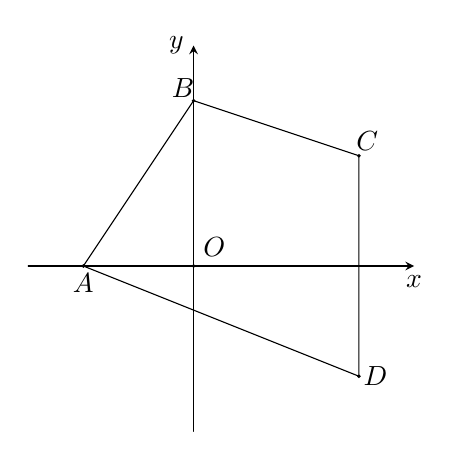
\begin{tikzpicture}[line join=round,line cap=round,>=stealth,scale=.7]
			\path 
				(-2,0)  coordinate (A)
				(0,3) coordinate  (B)
				(3,2) coordinate (C) 
				(3,-2)  coordinate (D);
			 \draw (A)--(B)--(C)--(D)--(A);
			 \draw[->] (-3,0)--(4,0) node[below]{$x$};
			\draw[->] (0,-3)--(0,4) node[left]{$y$}; 
			\fill (0,0) circle (1pt) node[above right]{$O$}; 
			\foreach \x/\g in {A/-90,B/130,C/60,D/0}\fill[black] (\x) circle (1pt)+(\g:3mm) node{$ \x $}; 
		\end{tikzpicture}
\end{center}
\shortans{3} 
\loigiai{Nhận thấy hình tứ giác $A B C D$ tính cả 4 cạnh của nó là miền nghiệm của hệ bất phương trình gồm 4 bất phương trình có miền nghiệm là nửa mặt phẳng chứa điểm $O(0; 0)$ và lần lượt có các bờ là các đường $A B$, $B C$, $C  D$ và $D A$.\\
	Phương trình đường thẳng $A B\colon-3  x+2 y=6$. Bất phương trình có miền nghiệm là nửa mặt phẳng bờ $A B$ (tính cả bờ $A B$) và chứa điểm $O(0; 0)$ là $-3 x+2 y \leq 6$.\\
	Phương trình đường thẳng $B C\colon x+3 y=9$. Bất phương trình có miền nghiệm là nửa mặt phẳng bờ $B C$ (tính cả bờ $B C$)  và chứa điểm $O(0; 0)$ là $x+3 y \leq 9$.\\
	Phương trình đường thẳng $C D\colon  x=3$. Bất phương trình có miền nghiệm là nửa mặt phẳng bờ $C D$ (tính cả bờ $C D)$ và chứa điểm $O(0; 0)$ là $x \leq 3$.\\
	Phương trình đường thẳng $D A\colon 2 x+5 y=-4$. Bất phương trình có miền nghiệm là nửa mặt phẳng bờ $D A$ (tính cả bờ $D A$) và chứa điểm $O(0; 0)$ là $2 x+5  y \geq-4$.\\
	Như vậy tứ giác $A B C D$ tính cả 4 cạnh của nó là miền nghiệm của hệ bất phương trình \begin{center}
	 $\heva{&-3 x+2 y \leq 6\\&x+3 y \leq 9\\&x \leq 3\\&2 x+5 y \geq-4}$ (*)
	\end{center}.\\ Điểm $M(m; m+1)$ nằm trên hình tứ giác $ABCD$ tính cả bốn cạnh của nó khi và chỉ khi $(m; m+1)$ là một nghiệm của hệ $(*)$, tức là
	 $$
	 \heva{
	&- 3 m + 2 ( m + 1) \leq 6  \\
	& m + 3 (  m + 1) \leq 9 \\
	&  m \leq 3 \\
	&2 m + 5  ( m + 1) \geq - 4 }
	\Leftrightarrow \heva{ 
	&m \geq-4 \\ 
	&m \leq  \dfrac{3}{2} \\
	&m \leq 3  \\
	&m \geq-\dfrac{9}{7}} 
	\Leftrightarrow-\dfrac{9}{7} \leq m \leq \dfrac{3}{2} \xrightarrow{m \in \mathbb{Z}} m \in\{-1; 0; 1\} 
	 $$
 }
\end{bt}


%%%%%%%%%%%%%%%% TỰ LUẬN %%%%%%%%%%%%%%%%

% nguồn: MaHoaNH_TuLuan_Lop10
\begin{bt}%[0D2V2-2]%[ma:8a509aa5]
	 Tìm các cặp số $(x;y)$ là nghiệm của hệ bất phương trình sau:
	\begin{enumEX}[a)]{2}
		\item $\heva{&2x-5\le 0 \\&-y+1\ge 0 \\ &3x+y\le 4}$ trong đó $x\in \mathbb{N}$, $y\in  \mathbb{N}$;
		\item $\heva{&x >  0 \\&2x-4\le 0 \\&y-1< 0 \\&2x+1> 0}$ trong đó $x\in \mathbb{Z}$, $y\in \mathbb{Z}$.
	\end{enumEX}
	\loigiai{ 
		\begin{enumEX}[a)]{1}
			\item Ta có $2x-5\le 0\Leftrightarrow x\le \dfrac{5}{2}$, do $x\in  \mathbb{N}\Rightarrow x\in \left\{0;1;2\right\}$.\\
			$-y+1\ge  0\Leftrightarrow y\le 1$, do $y\in \mathbb{N}\Rightarrow y\in \left\{0;1\right\}$.\\
			Mặt khác $3x+y\le 4$ nên  suy ra $\heva{&x=0 \\
			&y=0};\heva{&x=0\\&y=1}$; $\heva{&x=1 \\&y=0}$; $\heva{&x=0 \\&y=1.}$\\ 
			Vậy các cặp số $(x;y)$, trong đó $x\in \mathbb{N}$, $y\in \mathbb{N}$ là nghiệm của hệ bất phương trình  đã cho là
			\[(0;0),(0;1),(1;0),(1;1).\] 
			\item Ta có $\heva{&x > 0 \\&2x-4\le  0} \Leftrightarrow 0< x\le 2$ do $x\in \mathbb{Z}\Rightarrow x\in \left\{1;2\right\}$.\\
			Do $\heva{&y-1< 0 \\&2y+3> 0} \Leftrightarrow \dfrac{-3}{2}  < y < 1$ do $y\in \mathbb{Z}\Rightarrow y\in \left\{-1;0\right\}$.\\
			Vậy các cặp số $(x;y)$, trong đó $x\in \mathbb{Z}$, $y\in \mathbb{Z}$ là nghiệm của  hệ bất phương trình đã cho là
			 \[(1;-1),(1;0),(2;-1),(2;0).\]
	\end{enumEX}}
\end{bt}

% nguồn: MaHoaNH_TuLuan_Lop10
\begin{bt}%[0D2V2-2]%[ma:63aa4177]
	Tìm giá trị lớn nhất của biểu thức $T(x;y)=20\cdot 4\cdot x+30\cdot 4\cdot(x+y)+25\cdot 4\cdot y$ với  điều kiện $\heva{&x\ge 6\\&y\ge 2x\\&x+y\ge 24\\&y\le 20.}$
	 \loigiai{
		Biểu diễn tập nghiệm của  hệ bất phương trình ta được:
		\begin{center}
			\begin{tikzpicture}[line join=round,line cap=round,>=stealth,thick]
					\tikzset{every  node/.style={scale=0.9}}
					\begin{scope}
						\clip  (-1,-1) rectangle (6,6);
						\fill[pattern=north east  lines]
						 (1.2,4)--(2,4)--(1.6,3.2)--(1.2,3.6)--cycle;
						\draw (-1,-2)--(3,6); 
						\draw  (-1,4)--(6,4);
						\draw  (1.2,-1)--(1.2,6);
						\draw (6,-1.2)--(-1,5.8); 
					\end{scope}
					\draw[->] (-1,0)--(7,0)  node[below]{$x$};
					\draw[->] (0,-1)--(0,6.2) node[left]{$y$}; 
					\draw  (0,0) node[below left]{$O$};
					\fill[black] (1.2,4) node[above right]{$A$}circle (1pt) 
						(2,4) node[below]{$B$}circle (1pt) 
						 (1.6,3.2) node[below]{$D$}circle (1pt)
						(1.2,3.6) node[left]{$C$}circle  (1pt);
				\end{tikzpicture}
		\end{center}
		Tập nghiệm của hệ bất  phương trình giới hạn bởi tứ giác $ABCD$ với:\\
		$A(6;20)$, $B(10;20)$, $C(8;16)$,  $D(6;18)$\\
		Vì $T(x;y)=20\cdot 4\cdot x+30\cdot 4\cdot(x+y)+25\cdot 4\cdot y$ nên ta có\\ 
		 $T(6;20)=20\cdot 4\cdot 6+30\cdot 4\cdot(6+20)+25\cdot 4\cdot 20=5\,600$\\
		$T(10;20)=20\cdot 4\cdot 10+30\cdot 4\cdot(10+20)+25\cdot  4\cdot 20=6\,400$\\
		$T(8;16)=20\cdot 4\cdot 8+30\cdot 4\cdot(8+16)+25\cdot  4\cdot 16=5\,120$\\
	$T(6;18)=20\cdot  4\cdot 6+30\cdot 4\cdot(6+18)+25\cdot 4\cdot 18=5\,160$}
\end{bt}

% nguồn: MaHoaNH_TuLuan_Lop10
\begin{bt}%[0D2V2-2]%[ma:c585f746]
	Tìm tổng tất cả các giá trị nguyên của tham số $m$ trong đoạn $[-10;10]$ để $2x-3y-m\ge 0$ với mọi cặp số $(x;y)$ thoả mãn hệ bất phương trình sau $\heva{&-2x+y\le 2\\&-x+2y\le 4\\&x+y\le 5\\&y\ge 0}$ \quad (1). 
	 \loigiai{
		Miền nghiệm của hệ bất phương trình  là miền tứ giác $ABCD$ với $A(-1;0),B(5;0),C(2;3)$, $D(0;2)$ (Hinh vẽ).
		\begin{center}
			\begin{tikzpicture}[scale=1.0,font=\footnotesize,line join=round,line cap=round,thick,>=stealth];
					\begin{scope}
						\clip (-5,-2) rectangle  (6,6);
						\fill[pattern=north east lines,opacity=0.5] (-5,-2)--(-5,6)--(6,6)--(6,-2)--cycle; 
						\fill[white]  (-1,0)--(0,2)--(2,3)--(5,0)--cycle;
						 \draw (-1,10)--(11,10)
						 (10,-1)--(10,12);
						\draw[samples=150,smooth,domain=-5:6] plot (\x,{2*(\x)+2}); 
						\draw[samples=150,smooth,domain=-5:6] plot  (\x,{0.5*(\x)+2});
						\draw[samples=150,smooth,domain=-5:6] plot  (\x,{-1*(\x)+5});
					\end{scope}
					\draw[->] (-5,0)--(6,0)  node[below]{$x$};
					\draw[->]  (0,-2)--(0,6) node[left]{$y$};
					\draw (0,0) node[below  left]{$O$};
					\foreach  \x in {-1,-2,-3,-4,1,2,3,4,5}
					 \draw[thin] (\x,1pt)--(\x,-1pt) node [below] {$\x$};
					 \foreach \y in {-1,1,2,3,4,5}
					\draw[thin]  (1pt,\y)--(-1pt,\y) node [left] {$\y$};
					\draw (-1,0)  node[above left]{$A$}
						(0,2)  node[below right]{$D$}
						 (2,3) node[above]{$C$}
						(5,0) node[above right]{$B$}; 
				\end{tikzpicture}
		\end{center}
		 Ta có $2x-3y-m\ge 0\Leftrightarrow 2x-3y\ge m$.\\
		Vậy để $2x-3y-m\ge 0$ với mọi cặp số $(x;y)$ thoả mãn hệ bất phương trình $(1)$ thì $m\le \min \left(2x-3y\right)$, với mọi cặp số $(x;y)$ thoả mãn hệ bất  phương trình $(1)$.\\
		Đặt  $F=2x-3y$.\\
		Tính giá trị của $F=2x-3y$  tại các cặp số $(x;y)$ là toạ độ của các đỉnh tứ giác $ABCD$.\\
		Ta có $F(-1;0)=-2$, $F(5;0)=10$, $F(2;3)=-5$, $F(0;2)=-6$.\\ 
		Suy  ra giá trị nhỏ nhất của $F$ là $-6$.\\
		Vậy $m\le-6$ mà $m$ nguyên trong đoạn $\left[-10;10\right]$ nên $m\in  \left\{-10;-9;-8;-7;-6\right\}$.\\
		 Tổng các giá trị nguyên cần tìm của $m$ là $-40$.
	 }
\end{bt}

% nguồn: MaHoaNH_TuLuan_Lop10
\begin{bt}%[0D2K2-2]%[ma:57e3abbf]
	Đội thanh niên xung kích nhà trường gồm$ 24 $học sinh có$ 7 $học sinh khối$ 12$, $8 $học sinh khối$ 11 $và$ 9 $học sinh khối$ 10 $. Lần này, nhà trường cần chọn ra$ 9 $học sinh trong đội xung kích để lao động dọn vệ sinh phòng chống dịch Covid-19, hỏi có bao nhiêu cách chọn  sao cho
	\begin{enumerate}
		\item Mỗi khối có  đúng$ 3 $học sinh.
		\item Mỗi khối có ít  nhất$ 1 $học sinh.
	\end{enumerate}
	\loigiai{ 
		\begin{enumerate}
			\item Ta có 
			\begin{itemize}
				\item  Chọn$ 3 $học sinh khối$ 12 $có$ \mathrm{C}_7^3 $cách.
				\item Chọn$ 3 $học sinh khối$ 11 $có$ \mathrm{C}_8^3  $cách.
				\item Chọn$ 3 $học sinh  khối$ 10 $có$ \mathrm{C}_9^3 $cách.
			\end{itemize}
			Vậy có$ \mathrm{C}_7^3\cdot\mathrm{C}_8^3\cdot\mathrm{C}_9^3=164640 $cách. 
			\item Chọn ngẫu nhiên$ 9 $học sinh thì  có$ \mathrm{C}_{24}^9 $cách.\\
			Trong  đó số cách chọn$ 9 $học sinh không đủ$ 3 $khối gồm$ 4 $trường hợp:
			\begin{itemize}
				\item Chọn$ 9 $học sinh  khối$ 10 $có$ \mathrm{C}_9^9 $cách.
				\item Chọn$ 9 $học sinh gồm khối$ 10 $và khối$ 11 $là$  \mathrm{C}_{17}^9-\mathrm{C}_9^9=243094 $cách.
				\item Chọn$  9 $học sinh gồm khối$ 11 $và khối$ 12 $là$ \mathrm{C}_{15}^9=5005 $cách.
				\item Chọn$ 9 $học sinh gồm khối$ 10  $và khối$ 12 $là$ \mathrm{C}_{16}^9-\mathrm{C}_9^9=11439 $cách.
			\end{itemize}
			Vậy có$ \mathrm{C}_{24}^9-1-24309-5005-11439=1266750  $cách.
		\end{enumerate}
	 }
\end{bt}

% nguồn: MaHoaNH_TuLuan_Lop10
\begin{bt}%[0D2K2-2]%[ma:cf2d4aa3]
	Bác Năm dự định trồng ngô và đậu xanh trên môt mảnh đất có diện tích 8 ha. Nếu trồng 1 ha ngô thì cần 20 ngày công và thu được 40 triệu đồng. Nếu trồng 1 ha đậu xanh thì cần 30 ngày công và thu được 50 triệu đồng. Bác Năm cần trồng bao nhiêu hecta cho mỗi loại cây để thu được nhiều tiền nhất? Biết rằng, bác Năm chỉ có thể sử dụng không quá 180 ngày công cho  việc trồng ngô và đậu xanh.
	 \loigiai{
		Gọi $x$ là số hecta đất trồng ngô và $y$ là số hecta đất trồng  đậu xanh. Ta có các điều kiện ràng buộc đối với $x, y$ như sau
		\begin{itemize}
			\item Hiển nhiên $x \geq 0,  y \geq 0$.
			\item Diện tích canh tác không vượt quá 8 ha nên $x+y \leq  8$.
			\item Số ngày công sử dụng không vượt quá 180 nên $20x+30y  \leq 180$.
		\end{itemize}
		Từ đó, ta có hệ bất phương trình mô tả các  điều kiện ràng buộc:
		$\heva{&x+y \leq 8 \\& 20x+30y \leq 180 \\& x \geq 0 \\& y  \geq 0.}$\\
	\immini{Biểu diễn  miền nghiệm của hệ bất phương trình này trên hệ truc toạ độ $Oxy$, ta được miền tứ giác $OABC$.\\
		Tọa độ các đỉnh của tứ giác đó là: $O(0;0); A(0;6)$;  $B(6;2); C(8;0)$.\\
		Gọi $F$ là số tiền (đơn vị: triệu đồng) bác Năm thu được, ta có: $F=40x+50y$.\\ 
		Ta phải tìm $x, y$ thỏa mãn hệ bất phương trình sao cho $F$ đạt giá trị lớn nhất, nghĩa là tìm  giá trị lớn nhất của biểu thức $F=40x+50y$ trên miền tứ giác $OABC$.\\
		 }{
		\begin{tikzpicture}[line join=round,line cap=round,>=stealth,thick,scale=0.8]
				\tikzset{label  style/.style={font=\footnotesize}}
				\begin{scope}
					\clip  (-1,-1) rectangle (10,10);
					\fill[pattern=north east lines] (-3,11)--(11,11)--(11,-3)--cycle; 
					\fill[pattern=north east lines] (-7,10.67)--(11,10.67)--(11,-1.33)--cycle; 
					\fill[pattern=north east  lines] (0,-1)--(-1,-1)--(-1,10)--(0,10)--cycle;
					\fill[pattern=north east lines] (-1,0)--(-1,-1)--(10,-1)--(10,0)--cycle; 
					\draw  (-2,10)--(9,-1) node [pos=0.45,above,sloped] {$x+y-8=0$};
					\draw  (-6,10)--(10.5,-1) node [pos=0.55,below,sloped] {$20x + 30y -180=0$};
				\end{scope}
				 \draw[->] (-1,0)--(10,0) node[below]{$x$};
				 \draw[->] (0,-1)--(0,10) node[left]{$y$};
				\draw  (0,0) node[below left]{$O$}
					(0,8) node[right]{$8$} 
					(0,6) node[left]{$6$} 
					(0,6)  node[right]{$A$}
					(8,0)  node[below]{$8$}
					(9,0) node[below]{$9$} 
					 (6,2) node[above]{$B$}
					(8,0) node[above]{$C$}; 
				\draw[dashed](6,0) node[below]{$6$}--(6,2)--(0,2)  node[left]{$2$};
			\end{tikzpicture}
		} 
		 \noindent
		 Tính các giá trị của biểu thức $F$ tại các đỉnh của đa giác, ta có:\\
		Tại $O(0;0): F=40\cdot 0+50\cdot  0=0$.\\
		Tại  $A(0;6): F=40\cdot 0+50\cdot 6=300$.\\
		Tại $B(6;2): F=40\cdot 6+50\cdot 2=340$.\\ 
		Tại $C(8;0): F=40\cdot  8+50\cdot 0=320$.\\
		 $F$ đạt giá trị lớn nhất bằng 340 tại $B(6;2)$.\\
		Vậy để thu được nhiều tiền nhất, bác Năm cần trồng 6  ha ngô và 2 ha đậu xanh.
	} 
\end{bt}

% nguồn: MaHoaNH_TuLuan_Lop10
\begin{bt}%[0D2K2-2]%[ma:ce7060f9]
	Một người dùng ba loại nguyên liệu $A, B, C$ để sản xuất ra hai loại sản phẩm $P$ và $Q$. Để sản xuất $1 \mathrm{kg}$ mỗi loại sản phẩm $P$ hoặc $Q$ phải dùng một số kilôgam nguyên liệu khác nhau. Tổng số kilôgam nguyên liệu mỗi loại mà người đó có và số kilôgam từng loại nguyên liệu cần thiết để sản xuất ra $1 \mathrm{kg}$ sản phẩm mỗi loại được cho trong bảng  sau:
	\begin{center}
		\begin{tikzpicture}[>=stealth,line join=round,line cap=round,scale=1]
				 \draw (0.25,-.5) node{Loại nguyên liệu}
					 (4,-.25) node{Số kilôgam}
					(10,0.1) node{Số kilôgam  từng loại nguyên liệu}
					(4,-.75) node{nguyên  liệu đang có}
					(10,-0.4) node{cần để sản xuất 1kg sản phẩm} 
					 (8,-1.25) node{$P$}
					(12,-1.25) node{$Q$} 
					(0.25,-2) node{$A$} 
					(0.25,-3) node{$B$} 
					(0.25,-4) node{$C$} 
					(4,-2) node{$10$} 
					(4,-3)  node{$4$}
					(4,-4)  node{$12$}
					(8,-2)  node{$2$}
					 (8,-3) node{$0$}
					 (8,-4) node{$2$}
					 (12,-2) node{$2$}
					 (12,-3) node{$2$}
					 (12,-4) node{$4$};
				 \draw (-1.5,.5)--(14,0.5)--(14,-4.5)--(-1.5,-4.5)--cycle (2,0.5)--(2,-4.5)
					 (6,.5)--(6,-4.5)
					 (10,-.75)--(10,-4.5)
					 (-1.5,-1.5)--(14,-1.5)
					 (6,-.75)--(14,-.75)
					(-1.5,-2.5)--(14,-2.5) 
					 (-1.5,-3.5)--(14,-3.5);
			\end{tikzpicture}
	\end{center}
	Biết 1kg sản phẩm $P$ có lợi nhuận 3 triệu đồng và 1kg sản  phẩm $Q$ có lợi nhuận 5 triệu đồng. Hãy lập phương án sản xuất hai loại sản phẩm trên sao cho có lãi cao nhất.
	\loigiai{ 
	\immini{Gọi  $x$ là số kilôgam sản phẩm $P$, $y$ là số kilôgam sản phẩm $Q$ cần sản xuất. Ta có hệ bất phương trình:
		$\heva{&2x+2y \leq 10 \\&2y \leq 4 \\&2x+4y \leq 12 \\&x \geq  0 \\&y \geq 0.}$\\
		Biểu diễn miền nghiệm của hệ bất phương trình trên hệ trục tọa độ $Oxy$, ta được như hình bên. 
		 }{
		\begin{tikzpicture}[line join=round,line cap=round,>=stealth,thick]
				\tikzset{label style/.style={font=\footnotesize}} 
				\begin{scope}
					\clip (-1,-1) rectangle  (8,6);
					\fill[pattern=north  east lines] (-2,7)--(9,7)--(9,-4)--cycle;
					\fill[pattern=north east lines]  (-1,2)--(-1,6)--(8,6)--(8,2)--cycle;
					\fill[pattern=north east lines] (-7,6.5)--(9,6.5)--(9,-1.5)--cycle; 
					\fill[pattern=north east  lines] (0,-1)--(-1,-1)--(-1,6)--(0,6)--cycle;
					\fill[pattern=north east lines] (-1,0)--(-1,-1)--(8,-1)--(8,0)--cycle; 
					\draw (-1,6)--(6,-1)  node [pos=0.45,above,sloped] {$2x+2y=10$};
					\draw  (-1,2)--(8,2) node [pos=0.7,above,sloped] {$2y=4$};
					 \draw (-6,6)--(8,-1) node [pos=0.45,above,sloped] {$2x+4y=12$};
				\end{scope}
				\draw[->] (-1,0)--(8,0)  node[below]{$x$};
				 \draw[->] (0,-1)--(0,6) node[left]{$y$};
				\draw (0,0) node[below  left]{$O$}
					(0,2) node[below  left]{$2$}
					(0,2) node[below right]{$C$} 
					 (2,2) node[below]{$B$}
					(4,1)  node[below]{$A$}
					 (5,0) node[above]{$D$}
					(5,0)  node[below]{$5$};
			\end{tikzpicture}
		} 
		\noindent 
		Miền nghiệm là miền ngũ giác $OCBAD$ (hình trên) với các  đỉnh: $O(0;0); C(0;2); B(2;2)$; $A(4;1); D(5;0)$.\\
		 Gọi $F$ là số tiền lãi (đơn vị: triệu đồng) thu được, ta có: $F=3x+5y$.\\
		 Tính giá trị của $F$ tại các đỉnh của ngũ giác:
		\begin{enumEX}[\faCheckSquareO]{2}
			 \item Tại $O(0;0): F=3\cdot 0+5\cdot 0=0$.
			\item Tại  $C(0;2): F=3\cdot 0+5\cdot 2=10$.
			\item Tại $B(2;2): F=3\cdot 2+5\cdot 2=16$. 
			\item Tại $A(4;1): F=3\cdot  4+5\cdot 1=17$.
			 \item Tại $D(5;0): F=3\cdot 5+5\cdot 0=15$.
		\end{enumEX}
		$F$ đạt giá trị lớn  nhất bằng 17 tại $A(4;1)$.\\
		Vậy người đó cần sản xuất $4 \mathrm{kg}$ sản phẩm  $P$ và $1 \mathrm{kg}$ sản phẩm $Q$ để có lãi cao nhất là 17 triệu đồng.
	} 
\end{bt}
